\PassOptionsToPackage{table,xcdraw}{xcolor}
\documentclass{style}
\usepackage[utf8]{inputenc}
\usepackage[T1]{fontenc}
\usepackage{amsmath}
\usepackage{amssymb}
\usepackage{tikz}
\usepackage{gensymb}
\usepackage[Algorithme]{algorithm}
%\usepackage{algorithmicx}
\usepackage{systeme,mathtools}
\usepackage{listings}
\usepackage{booktabs}
\usepackage[nounderscore]{syntax}
\usepackage{graphicx}
\usepackage{caption}
\usepackage{subcaption}

\usepackage{wrapfig}

%--------------------------------------------------------
%	 PAGE DE TITRE
%--------------------------------------------------------

\title{PFA}
\lesoustitre{Packing d'images vectorielles}

\discipline{Génie logiciel}

\author{
%\begin{minipage}{4cm}
    Dorian Cuquemelle\\ 
    Élodie Feng\\
    Hugo Le Dily \\
    Maxime Mondot\\
    Youssef Naim\\
    Virgile Robles\\
    Adrien Rodrigues
%\end{minipage}
}

\nomdeuniversite{ENSEIRB-MATMECA}

\unite{Département informatique 2ème année}
\ecoledoc{ENSEIRB-MATMECA}
\logouniversite{img/enseirb.png}
\scalelogouniversite{0.4}
\logoprojet{img/vertebrae.png}
\scalelogoprojet{0.6}

\encadrant{J. Allali} 
\client{D. Renault}

%--------------------------------------------------------
%	 BEGIN DOCUMENT
%--------------------------------------------------------
\begin{document}
\justifying
\maketitle
\newpage

\tableofcontents
\newpage

%--------------------------------------------------------
%	 INTRODUCTION
%--------------------------------------------------------
\section*{Introduction}
%Introduction

Dans le cadre de l'enseignement de 2ème année informatique de l'ENSEIRB-MATMECA, nous avons été amenés à travailler en équipe de sept étudiants sur un projet de longue durée. L'objectif était d'une part de développer nos compétences techniques, mais également et principalement de nous confronter à des problématiques s'apparentant à celles rencontrées en entreprise, telles que le contact client et la méthodologie de travail de groupe.\\

L'utilisation de machines de découpe de matériaux telle que la découpeuse laser est de plus en plus répandue parmi les \texttt{fablabs}, leur permettant un prototypage simple, rapide et automatisé. Inévitablement, un besoin d'économiser le matériau naît, et avec lui la volonté d'optimiser la disposition des pièces à découper sur la surface donnée. Comme il n'est pas évident de réaliser cette tâche manuellement, nous avons été chargés de trouver une solution pour l'automatiser de la meilleure manière possible.

Ce rapport présente dans un premier temps le contexte de ce projet et la méthodologie de travail que nous avons adoptée, puis dans un second temps la réponse que nous avons apportée à ce problème.


%\newpage

%--------------------------------------------------------
%	 CONTEXTE
%--------------------------------------------------------
\section{Contexte}
%----------------------------- LE CLIENT ----------------------------- 
\subsection{Le client}

% Logo Eirlab
\begin{center}

\includegraphics[scale=0.11]{img/eirlab_logo.png}
\end{center}

Ce projet est initié par Eirlab, le FabLab de l'ENSEIRB-MATMECA/Bordeaux INP. Il s'agit d'un atelier de fabrication numérique mettant à disposition de ses membres des outils de prototypage rapide. Les locaux de l'atelier se trouvent dans l'école ENSEIRB-MATMECA, à Talence.

L'atelier a ouvert au printemps 2016, il est plus particulièrement régi par l'association Eirlab Community. Cette dernière a pour objet la gestion, l'animation et la promotion de l'espace Eirlab à travers des évènements, formations gratuites ou payantes. L'association propose également un service de vente de matériaux pour les réalisations.

Peuvent adhérer au club personnes physiques, étudiantes de Bordeaux INP ou non, et personnes morales. 

Eirlab dispose de 400m² d'espace \textit{innovation} d'une part avec des stations de travail, et espaces de discussion, et espace de \textit{prototypage} d'autre part. Ce dernier met à disposition de ses membres six imprimantes 3D, une machine de découpe et gravure laser, une perceuse colonne, et autres outils électroniques et mécaniques. 

Le client est représenté par M. David RENAULT, comme initiateur du projet et principal interlocuteur pour les prises de décisions et validation du travail accompli. 


%----------------------------- LE BESOIN ----------------------------- 
\subsection{Description du besoin}

Le projet se place dans le cadre de l'utilisation de la machine de découpe/gravure laser pour usiner des pièces en deux dimensions.

\subsubsection*{Description de l'existant}

\begin{wrapfigure}{r}{6cm}
    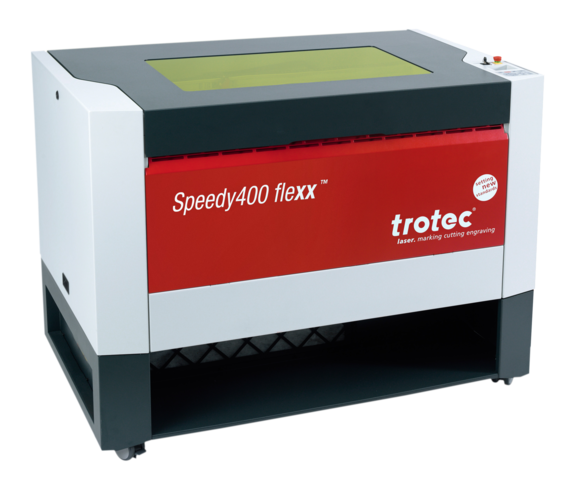
\includegraphics[scale=0.3]{img/lasermachine.png}
    \caption{Machine laser 400 Flexx Trotec}
    \label{fig:lasermachine}
\end{wrapfigure}

La machine présente à l'atelier est le modèle 400 Flexx de Trotec, elle permet de graver de nombreux matériaux, et de découper ou marquer certains d'entre eux. 

L'envoi de travaux à la machine se fait depuis le poste de travail à côté de celle-ci, depuis le logiciel de conception en passant par le logiciel de contrôle d'impression propriétaire \textit{JobControl}. L'usage à Eirlab est d'utiliser le logiciel \textit{Inkscape} pour éditer les fichiers vectoriels SVG à découper/graver.


\subsubsection*{Besoins du client}
Afin d'optimiser le temps de découpe et d'économiser les matériaux, le client souhaite faire intervenir un algorithme de \textit{packing} avant lancement de la découpe. Il s'agit de calculer une disposition des pièces à découper occupant le moins d'espace possible. Cette étape est pour le moment réalisée manuellement, ce qui est fastidieux pour l'utilisateur, et n'assure pas l'optimalité de l'agencement choisi. Voici un exemple en figure \ref{fig:before_after_pack} fichier source et de résultat attendu :

\begin{figure}[!htb] 
    \centering
    
\includegraphics[scale=0.12]{img/verteall.png}
    \caption{Exemple de packing attendu}
    \label{fig:before_after_pack}
\end{figure}

La figure \ref{fig:schema_besoin} suivante représente les différentes étapes traversées lors de l'utilisation de la découpeuse laser. Notre projet doit donc s'inscrire au niveau de l'étape d'édition du fichier vectoriel dans le logiciel Inkscape. 

\begin{figure}[H]
    \centering
    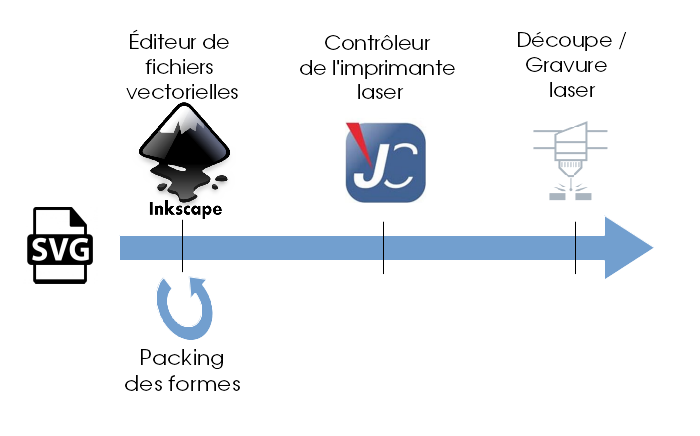
\includegraphics[scale=0.6]{img/schema_besoin.png}
    \caption{Schéma des étapes du cas d'utilisation général souhaité pour la découpe laser}
    \label{fig:schema_besoin}
\end{figure}



%% ------------ LE SUJET ------------ %%

\subsection{Le sujet}

Le client a souhaité que soit fourni un plug-in pour le logiciel Inkscape, depuis lequel il puisse déclencher les fonctionnalités de \textit{packing} développées dans notre solution, en plus de l'application depuis le terminal.

Il nous a été demandé de mettre en place un ensemble d'algorithmes réalisant de différentes manières une solution au problème de \textit{packing}. Ces derniers doivent pouvoir être lancés en parallèle, reprendre la solution de l'un comme entrée de l'autre etc., en somme, garantir une certaine modularité dans leur utilisation.



%Notre tâche première pour répondre aux besoins du client a été d'implémenter une base de solveur qui travaille avec des données vectorielles, avec le plug-in Inkscape associé pour une utilisation facile.

%Une fois les fondations de notre travail bien posées, il a fallu nous attaquer au solveur, qui regroupe des algorithmes de packing.
%Ces algorithmes seront de plus en plus complexes dans le but d'obtenir des résultats les plus efficaces possibles. On note par exemple la différence entre les algorithmes ne s'occupant que de rectangles par opposition à ceux qui gèrent l'imbrication de pièces.

%Il nous faut ensuite optimiser ce solveur afin que les algorithmes soient répartis efficacement sur les divers processeurs de la machine.

\subsubsection{Le problème de Bin-Packing}
La problématique d'optimiser l'espace et le nombre de planches utilisées constitue une instance d'un problème de bin-packing.\\

Le bin-packing est un problème relevant de l'optimisation combinatoire, ou il s'agit de ranger des objets de tailles $c_{1}, c_{2}, ... , c_{n}$ dans le minimum de boites de taille $C$(correspondant à des plaques dans notre cas).\\

Ce problème est présent dans plusieurs secteurs d'activité tels que le rangement de fichier dans un système informatique ou le découpage du verre.

Le problème de Bin-Packing est NP-difficile, donc à part pour les problèmes de tailles très réduites, les méthodes de résolutions sont principalement heuristiques et métaheuristiques.\\

Les méthodes heuristiques les plus utilisées de nos jours sont :  
\begin{itemize}
    \item \textit{first-fit decreasing (FFD)}: qui consiste à trier les objets dans un ordre décroissant de taille, puis pour chaque objet, on le range dans la première boite qui peut le contenir. 
    \item \textit{best-fit decreasing (BFD)}: le même tri qu'auparavant, sauf qu'on range l'objet dans la boîte la plus remplie qui puisse le contenir.
\end{itemize}
~\\

Plusieurs articles et thèses existent pour ce problème se basant sur différentes techniques d'optimisation telle que le branch and bound:\\

\textit{  Two-Dimensional Finite Bin-Packing Algorithms J. O. Berkey and P. Y. Wang The Journal of the Operational Research Society Vol. 38, No. 5 (May, 1987), pp. 423-429  ) }\\

\textit{A Genetic Algorithm for a 2D Industrial Packing Problem E. Hopper, B. Turton University of Wales, Cardiff, Computers and Industrial Engineering, vol. 37/1-2, pp. 375-378, 1999. }\\


%--------------------------------------------------------
%	 MÉTHODOLOGIE ET OUTILS
%--------------------------------------------------------
\section{Méthodologie et outils de programmation}
%% PARTIE 3 : Méthodologie et outils de développement

\subsection{Méthode Kanban}

La réalisation du projet a été faite en suivant la méthode Kanban, une méthode agile et itérative. La méthode consiste notamment à représenter les tâches composant le projet sur un tableau en plusieurs colonnes afin que tous les participants puissent suivre l'avancement de ce dernier.\\

Comme plusieurs autres méthodes agiles, elle repose sur le concept d'\textit{User Story} (U.S.). Cette expression désigne un besoin exprimé du point de vue du client, qu'on peut mettre sous la forme \textit{En tant que [...], je veux [...] afin de [...]}, que le développeur est chargé de réaliser.\\

Le fait de représenter l'ensemble des tâches à réaliser par le développeur sous forme d'U.S. impose de toujours voir le projet du point de vue du client, ce qui permet de rester pertinent sur ce qui est développé. Une U.S. commence à l'extrémité gauche du tableau, et se déplace vers la droite au fur et à mesure qu'elle passe les différentes étapes de réalisation, pour finir à l'extrémité droite lorsqu'elle est validée (indépendemment de ses opinions politiques).\\

La méthode Kanban, à l'inverse d'une méthode comme SCRUM, ne fonctionne pas par cycles mais en flux tendu : au lieu d'avoir un certain nombre d'U.S. à réaliser toutes les $x$ semaines, on se fixe un nombre minimal et maximal d'U.S. qui doivent être en cours de réalisation à tout moment. Ces nombres sont choisis en fonction de la capacité de travail de l'équipe de développement.\\

De plus, à toute U.S. doit être attribuée une difficulté de réalisation ainsi qu'une valeur client (utilité), qui sont des valeurs sur une échelle de Fibonacci (puisqu'il est contre-productif d'être extrêmement précis dessus). On utilise alors ces deux valeurs pour déterminer quelles U.S. réaliser parmi celles qui sont spécifiées, en prenant par exemple celles qui ont le plus grand ratio \textit{utilité/difficulté}.\\

Nous avons choisi de mettre dans notre tableau les colonnes suivantes (entre autres) :
\begin{itemize}
    \item \textbf{Product backlog} : c'est ici qu'apparaissent toutes les U.S. du projet à leur création, ainsi que les idées d'ordre plus général, issues de divers brainstorming.
    
    \item \textbf{U.S. "INVEST"} : recense toutes les U.S. mises au format "INVEST" : pour chacune, des niveaux de difficulté technique et de valeur marchandes ont été déterminés. C'est donc la liste des U.S. normalisées à faire, susceptibles de passer à la réalisation.
    
    \item \textbf{U.S. en cours} : liste les U.S. en cours de réalisation. Le nombre d'U.S. dans cette colonne est limité afin de ne pas surcharger les collaborateurs du projet. Chaque U.S. doit à ce niveau là être attribuée à une partie de l'équipe.
    
    \item \textbf{Révision} : contient les U.S. dont l'implémentation est finie mais à faire réviser par d'autres membres de l'équipe pour la logique, la lisibilité, les commentaires et plus généralement la qualité du code écrit.
    
    \item \textbf{Démo} : stocke les U.S. validées par l'équipe mais pas encore par le client. C'est la dernière étape avant qu'une U.S. soit définitivement réalisée et archivée.
\end{itemize}
Nous avons exploité le site \textit{kanboard.ipb.fr} pour travailler sur ce tableau, dont un peu voir un aperçu en figure~\ref{fig:kanboard}.

\begin{figure*}[!htb]
    \centering
    \begin{subfigure}{.8\linewidth}
        \centering
        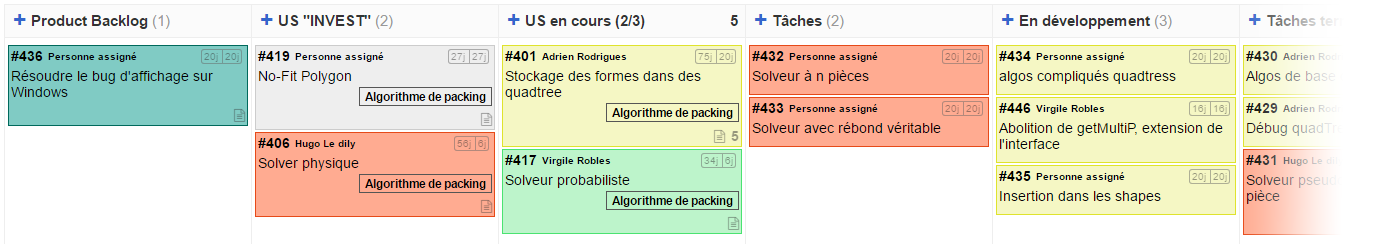
\includegraphics[width=\linewidth]{img/kanboard01.png}
    \end{subfigure}%
    ~ \\
    \begin{subfigure}{.8\linewidth}
        \centering
        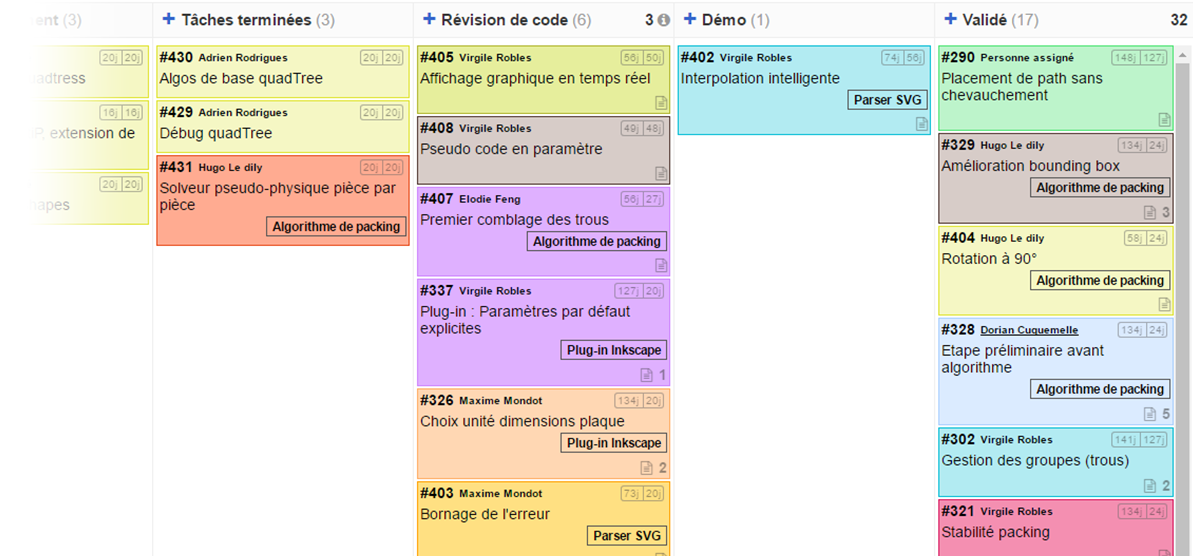
\includegraphics[width=\linewidth]{img/kanboard02.png}
    \end{subfigure}
    \caption{Aperçu de notre Kanboard}
    \label{fig:kanboard}
\end{figure*}


\subsection{La méthode dans les faits}

L'organisation du travail en équipe s'est déroulée comme suit:
\begin{itemize}
    \item A chaque réunion avec le client et/ou le responsable pédagogique, nous présentions notre travail hebdomadaire, avec démonstration d'une exécution fonctionnelle lorsque cela s'avérait pertinent.
    \item A l'issue de la réunion, nous organisions les nouvelles tâches à réaliser sous forme de nouveaux éléments dans le product backlog et d'User Stories dans notre Kanban.
    \item Ensuite, les membres de l'équipe s'accordaient à travailler en petits groupes sur plusieurs nouvelles U.S., ou continuaient à travailler sur celles qui n'avaient pas été complétées lors de la semaine.\\    
\end{itemize}

Nous avons apprécié la méthode Kanban car l'agilité nous a permis de confronter régulièrement notre avancement avec les besoins du client et ainsi de mettre à jour les attentes prioritaires, de prendre en compte ses remarques vis à vis de notre vision du sujet pour éviter les mauvaises interprétations etc.\\

%METTRE LES PROBLEMES PLUS TARD QUAND MEME...

% 1. Pourquoi ca a pas marché
% 2. Qu'est ce qu'on changerait si on devait refaire 

Nous avons cependant eu quelques légers problèmes de travail en équipe.\\

Conserver une bonne méthodologie, particulièrement pour ce qui est d'une mise-à-jour régulière du Kanban, a parfois été négligé par certains aspects : Les membres de l'équipe communiquant sur l'avancement du projet en dehors des U.S. du Kanboard, ce dernier pouvait ne pas être mis à jour systématiquement. Cet écart à la méthode s'est également manifesté par l'abandon de l'attribution des business value et des difficultés aux User Stories, la perte de la division des U.S. en tâches et la création d'U.S. de manière mal organisée.\\

De plus, le PFA était un projet réalisé en \texttt{C++}, langage appris en même temps que le début du projet. La différence d'expérience en programmation des différents membres de l'équipe se ressentait sur la contribution sur le travail au départ, car certaines personnes étaient déjà habituées à ce langage, et d'autres non.\\

Plus précisément, l'environnement de développement du projet ne favorisait pas celui-ci. En effet, dans le contexte de notre formation, nous avions de nombreux autres projets et examens, nous empêchant de nous consacrer à ce travail aussi régulièrement que l'exige la méthode. Cela met en valeur un problème intrinsèque du PFA : effectuer un travail d'entreprise dans un contexte d'école d'ingénieurs. Il est impossible de se réunir tous les matins pour faire le point sur l'avancement de chacun, de travailler en pair-programming du fait de la différence des emplois du temps de chacun etc.\\

Dans une autre mesure, il s'agissait pour tous de notre première expérience dans un projet à long terme, et avec une équipe aussi grande. La communication est un aspect essentiel au bon fonctionnement d'un projet. Mais, par manque de savoir-faire, celle-ci a parfois était imparfaite, si bien que cela a pu nous ralentir, voire empêcher la compréhension mutuelle. \\ 

%Application du Kanban
%Diff d'experience code des membres
%Première experience grand projet
%Adaptation PFA dans le cadre de l'école : réunions régulières, examens, autres projets
%...

Ces problèmes de gestion d'équipe rencontrés nous ont permis de mieux comprendre l'importance de certains points. Si nous avions à refaire ce projet, nous chercherions une méthodologie plus adaptée à l'école, ou encore à adapter une certaine méthode à cet environnement, de sorte à garantir assez de rigueur pour un meilleur travail d'équipe. Le rôle du Scrum Master, membre de l'équipe chargé d'assurer l'application de la méthode par tous les membres, a été envisagé mais jamais mis en place. Il serait donc intéressant de revoir la structuration de l'équipe (un Scrum Master fixe ou à tour de rôle). La rétrospective hebdomadaire, réunion portant sur la méthode et non sur le projet en lui-même qui vise à déterminer ce qui fonctionne et ne fonctionne pas, et à trouver des solutions sous forme de plan d'action, pourrait également être mise en place, pour une amélioration continue de notre façon de travailler.\\


%La responsabilité de répartir le travail et de former les binômes a été, sur certaines occasions, laissée aux membres les plus inspirés quant à une U.S., les autres membres assistant ces développements.\\


%Enfin, les périodes de l'année chargées en examens ont fait quelque peu fluctuer le degré d'implication dans le PFA.\\

%Au début du PFA, il y a eu un problème principalement par rapport au niveau des membres en programmation et leur degrés de maîtrise du C++. Ce qui fait qu'il fut plus difficile pour certain de suivre la cadence. Cela s'est arrangé plus tard, lorsque on a avait fini les cours et TD en C++, et lorsque les membres les plus impliqués dans le code ont baissé un peu le rythme, et ont assuré des révisions de codes pour que tout le monde soit sur la même longueur d'onde.



\subsection{Outils}
Les outils utilisés pour la réalisation du produit sont :
\begin{itemize}
    \item Langage d'extension Inkscape
    \item Python : langage de programmation utilisé pour l'interface entre Inkscape et le solveur.
    \item C++ : langage de programmation pour le solveur
    \item CMake : outil permettant de gérer la compilation et l'installation des sources.
    \item Boost : ensemble de bibliothèques C++ utilisé ici pour parser les options passées au solveur
    \item svgpp : bibliothèque aidant au parsing de fichiers SVG
    \item rapidXML : bibliothèque de parsing de fichiers XML
    \item Doxygen : permet de générer la documentation à partir des commentaires sur les sources du produit
    \item mingw-w64 : ensemble d'outils permettant la cross compilation du produit pour Windows depuis Linux.
    
\end{itemize}

\vspace{1em}
Il a été choisi de développer le produit sur Linux à l'aide de la collection de compilateurs GCC. Les plates-formes supportées sont Windows et Linux, les deux devant être compilées depuis Linux.

\subsection{Le format SVG}

\indent Les données représentant les formes à packer sont décrites sous le format SVG qui est une spécialisation du format XML. Ce format représente une arborescence de données utilisant des balises.\\

Un noeud est délimité par une balise ouvrante et une fermante, ou bien une balise seule. La balise peut contenir un ensemble d'attributs dépendant de son type. Si le noeud est sous la forme de balises ouvrantes/fermantes, il peut y avoir d'autres noeuds entre ces balises (ce sont alors des noeuds fils).\\
Un ensemble particulier de noeuds et d'attributs est utilisé lors de notre programme (un exemple de syntaxe SVG est visible en figure~\ref{fig:svg}.

\begin{itemize}
    \item \textbf{Paths} : Les \textit{paths}, et primitives de formes (\texttt{rectangle}, \texttt{circle}, ...). Ce sont les noeuds qui sont utilisés pour représenter un contour. Ils possèdent un attribut \texttt{d} qui contient l'ensemble des informations permettant de décrire ce contours, sous différentes formes : segments, courbes de Bézier, etc.
    \item \textbf{Matrices de transformations} Ce sont des attributs qui sont appliqués au \textit{path} du noeud courant ainsi que tous ses fils. Elles permettent de déplacer un objet sans modifier explicitement les coordonnées de ses points. Elles doivent donc être prises en compte lors de la lecture du fichier. Nous les utilisons également pour appliquer les déplacement effectués par le programme dans le fichier de sortie.
    \item \textbf{Groupes} : Ils forment des ensembles d'objets qui peuvent se comporter comme une entité unique, et sont particulièrement utilisés pour la gestion des formes à trous ou lors de la génération du fichier de sortie (pour délimiter les différentes plaques).
    \item \textbf{Identifiants} : Les noeuds possèdent généralement un attribut \texttt{ID}. Ils permettent d'identifier rapidement un objet, chaque objet ayant une valeur unique pour cet attribut. Celui-ci peut être modifié lors de la génération du fichier de sortie en cas de duplication des objets.
    \item \textbf{Width}/\textbf{Height}/\textbf{Viewbox} : Ce sont des attributs propre au fichier. Ils sont utilisés pour déterminer les dimensions d'une plaque par défaut, ils peuvent être exprimés dans différentes unités, qu'il nous faut donc convertir au préalable dans une unité universelle utilisable par le programme.
\end{itemize}

\begin{figure}[H]
\centering
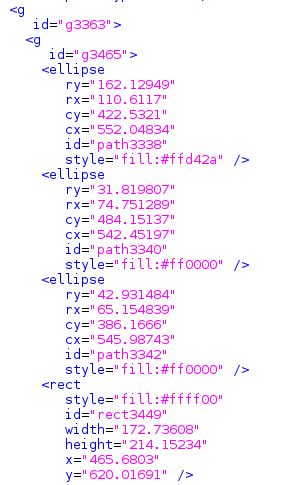
\includegraphics[scale=0.6]{img/svg.png}
\caption{Un morceau de fichier SVG}
\label{fig:svg}
\end{figure}



%--------------------------------------------------------
%	 ARCHITECTURE
%--------------------------------------------------------
\section{Architecture}
\subsection{Fonctionnement général}
Le projet, comme évoqué précédemment, s'articule autour de deux parties : le plugin \texttt{Inkscape} et les algorithmes.\\

Le plugin \texttt{Inkscape}, décrit plus en détail par la suite, envoie à un script Python un certain nombre d'arguments bruts. Ce dernier est chargé d'interpréter les arguments d'Inkscape et de les convertir (notamment au niveau des unités) en un format accepté par notre programme, qu'il appelle avec ces nouveaux arguments.

Ce programme, le solveur reçoit un fichier \texttt{SVG} et les arguments, et renvoie un fichier  \texttt{SVG} résultat sur la sortie standard, qui est alors affiché par \texttt{Inkscape}.\\

La partie la plus importante du projet est ce programme, dont nous allons par la suite détailler l'architecture. Un diagramme de classe de ce programme est visible en figure~\ref{fig:diagramme}

\begin{figure}[!htb]
\centering
\includegraphics[scale=0.7]{img/ClassDiagram.png}
\caption{Diagramme de classe du programme principal}
\label{fig:diagramme}
\end{figure}

\subsection{Représentation interne (\texttt{Shape})}

Nous introduisons le concept de \texttt{Shape} (forme), que nous utiliserons par la suite. Il s'agit d'une classe représentant une forme interpolée. Elle peut représenter un ou plusieurs polygones non indépendants, potentiellement chacun composés de trous. En effet, cette classe contient un \texttt{MultiPolygon}, type de la librairie Boost, lequel contient plusieurs \texttt{Polygon}. Enfin ce dernier contient un \texttt{Ring} (polygone fermé) décrivant son contour, et potentiellement plusieurs autres décrivant ses trous. Nous verrons dans la partie sur le parseur \texttt{SVG} comment nous transformons le document en un ensemble de telles \texttt{Shapes}. Cette hiérarchie est illustrée en figure~\ref{fig:multipolygon}\\

\begin{figure}[!htb]
\centering
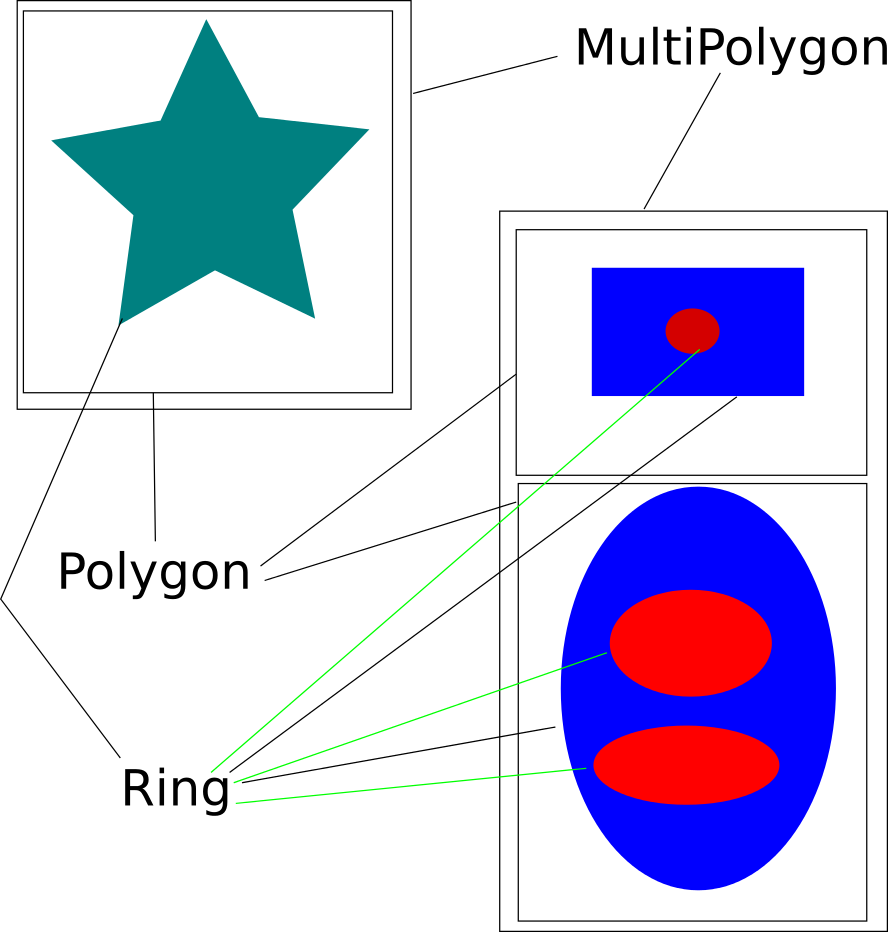
\includegraphics[scale=0.5]{img/MultiPolygon.png}
\caption{Hiérarchie \texttt{MultiPolygon}/\texttt{Polygon}/\texttt{Ring} (vert : \texttt{Ring} interne)}
\label{fig:multipolygon}
\end{figure}

Par la suite, il arrivera que faisions l'union de deux \texttt{Shapes} : il s'agit de générer un unique \texttt{MultiPolygon} contenant les \texttt{Polygons} de la première \textbf{et} la deuxième \texttt{Shape}. On parlera alors de \textit{bloc} de \texttt{Shapes} pour décrire une union (en effet faire l'union de deux \texttt{Shapes} revient à les considérer comme dépendantes l'une de l'autre : elles seront déplacées "ensemble").\\

Toutes ces formes sont stockées dans une classe \texttt{Layout}, qui décrit donc une disposition des pièces à un instant donné.\\

\subsection{Préparation des pièces}

Une fois les pièces générées, on commence par appliquer un \textit{buffer} sur ces dernières, c'est à dire augmenter leur épaisseur dans leur représentation interne. Ceci est utile non seulement pour compenser une erreur potentielle lors de l'interpolation des points, mais aussi si l'utilisateur souhaite une distance minimale entre les pièces une fois le packing réalisé. Le fait d'augmenter l'épaisseur en interne produira ce résultat, puisque les pièces seront positionnées comme si elles étaient plus épaisses, sans augmenter l'épaisseur réelle à la sortie.\\

\subsection{Choix concernant la sortie}

En effet nous avons choisi, lors de la génération du fichier de sortie, de ne pas créer de nouvelles formes à partir de notre représentation interne (potentiellement erronée), mais plutôt d'appliquer des transformations sur les formes originales. De cette manière on conserve l'ensemble des attributs donnés pour l'utilisateur.\\

Cela provoque quelques inconvénients : nous le verrons par la suite dans la classe \texttt{Outer}, mais celà nécessite (à cause de l'utilisation à l'entrée de \texttt{SVG++}) de parcourir une nouvelle fois le fichier original à la sortie.

\subsection{Fonctionnement interne des modules}

\subsubsection{Plug-In}

Afin de gérer l'interface entre Inkscape et notre programme, nous avons implémenté un plug-in python.
Celui-ci s'occupe de récupérer l'ensemble des paramètres transmis par Inkscape. Il effectue également un ensemble d'opérations permettant de convertir les unités de mesure en pixel, qui sont utilisables par notre programme. Il permet notamment d'extraire les dimensiona de la plaque depuis le fichier, puis de les convertir en pixel.\\
Pour réaliser ce travail nous avons utilisé la bibliothèque \texttt{inkex.py} fournie par Inkscape.\\



\subsubsection{Parser et SVG++}
%PARTIE SVG++%
Nous utilisons, pour lire le fichier d'entrée du programme, la bibliothèque \texttt{SVG++}.
Pour utiliser celle-ci, il faut définir un ensemble de comportements à adopter lors de la lecture des balises qui nous intéressent. Les méthodes implémentées au cours du projet sont visibles sur la figure~\ref{fig:SVGPP}.

\begin{figure}[H]
\centering
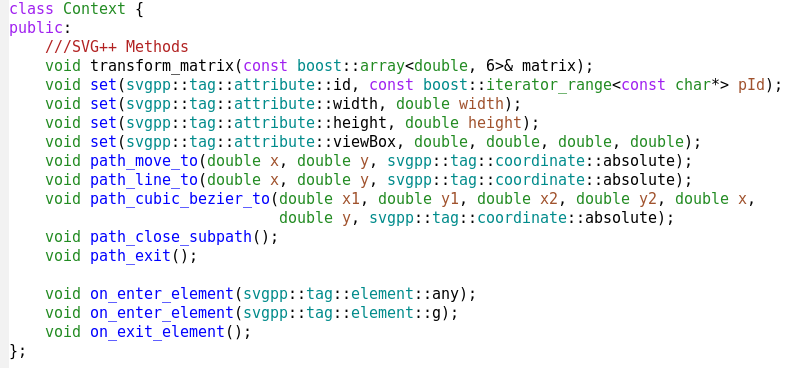
\includegraphics[scale=0.5]{img/SVGPP.png}
\caption{Méthodes à implémenter dans la classe Context de SVG++}
    \label{fig:SVGPP}
\end{figure}

Ces comportements peuvent être généralisés : par exemple, il est possible d'utiliser le comportement des courbes de Bézier sur tout les \texttt{path} rencontrés, la bibliothèque effectue alors la conversion nécessaire pour appliquer le comportement choisi.\\

Ceci permet notamment de ne pas gérer au cas par cas toutes les balises existantes, en ignorant celle n'étant pas utiles pour le bon fonctionnement du programme, et en utilisant un comportement générique pour une certaine variété de balises (\texttt{path}).\\

Cependant, l'implémentation de la bibliothèque est riche en métaprogrammation template.\\
La métaprogrammation est un outil permettant en particulier de générer du code à la compilation, par exemple, il est possible d'écrire une fonction avec un type générique qui sera ensuite déterminé lors de la compilation.\\
Il est également possible de pré-calculer des données lors de la compilation qui seront généralement stockées dans des variables statiques.\\
Ceci permet d'améliorer l'efficacité de certains programmes, et d'écrire du code plus générique. Cependant, les temps de compilations sont plus longs, les métaprogrammes sont assez peu lisibles et, en C++, il est impossible de redéfinir une méthode template dans une classe fille.\\

Il n'est alors pas possible d'utiliser le comportement habituel de la Programmation Orienté Objet (POO) (redéfinition de méthodes dans une classe fille), il est donc nécessaire de préciser quelles méthodes sont implémentées dans un ensemble utilisé par cette bibliothèque.\\
De plus celle-ci ne nous permet pas de stocker le contenu du fichier, nous devons donc ré-effectuer une lecture au moment de la génération du fichier de sortie. Et les temps de compilation sont fortement affectés.\\

%%END OF SVG++

%4. interpolation des courbes de Bézier
La grande majorité des formes étant décrites avec des courbes de Bézier, il était nécessaire d'avoir une méthode d'interpolation permettant d'obtenir des points à partir de ces courbes. La méthode d'interpolation la plus simple (nous avons par la suite utilisé une méthode plus intelligente, décrite par la suite) des courbes de Bézier en dimension 3 (puisque grâce à SVG++ toute courbe est ramenée à cette catégorie) est la suivante (avec ${\mathbf  {P}}_{0}$, ${\mathbf  {P}}_{1}$ et ${\mathbf  {P}}_{1}$ les points définissant la courbe de Bézier) :
$${\mathbf  {P}}(t)={\mathbf  {P}}_{0}(1-t)^{3}+3{\mathbf  {P}}_{1}t(1-t)^{2}+3{\mathbf  {P}}_{2}t^{2}(1-t)+{\mathbf  {P}}_{3}t^{3}, t \in [0, 1]$$\\
On fait varier $t$ avec un pas fixé pour obtenir $\frac{1}{t}$ points sur une courbe, qu'on insère dans les \texttt{Shapes}.\\

On obtient pour chaque \texttt{path} un polygone fermé (\texttt{Ring}). Il reste encore à répartir ces polygones dans des \texttt{Shapes}. Pour cela nous utilisons un algorithme qui trie les \texttt{Rings} par aire décroissante et teste la superposition des uns sur les autres, pour déterminer pour chaque \texttt{Ring} s'il s'agit d'un contour ou d'un trou.\\

De plus il faut décider si un ring fait partie d'un bloc : l'utilisateur a la possibilité de définir des ensembles de pièces qui seront déplacées ensembles en les mettant dans un \textbf{groupe} SVG. Il faut alors utiliser la présence des balises de groupe pour trier les polygones.

\subsubsection{Algorithmes de packing}

\paragraph{Transformers, Merger\\}

La classe \texttt{Transformer} est une classe abstraite pouvant adopter plusieurs comportements selon le Transformer choisi (Simple, Holes...). 
Cette classe s'occupe de déplacer plusieurs ensembles de Shapes qui seront ensuite considérés comme des 'blocs'.
Après déplacement des Shapes, le transformer retourne un vecteur contenant les vecteurs représentant les Shapes, liées par 'bloc'.

Cette variable de retour est ensuite récupérée par la classe Merger qui s'occupe de modifier la structure interne des données pour gérer les 'blocs' créés par le Transformer dans les algorithmes suivants (transformers et solvers). 

Lors de sa création, la classe Merger sauvegarde les informations nécessaires à la génération du fichier SVG. En effet, lors d'une phase de fusion, on ne considère que les points (ou quadtrees), eux seuls étant utiles aux algorithmes de packing. 

Afin de conserver l'intégrité de la représentation au cours de l'exécution, le merger stocke des ensembles d'identifiants indiquant à quelle forme appartenait un polygone (ou quadtree) à l'origine.

Un exemple de fonctionnement du merger est donné en figure \ref{fig:schemamerger}.

\begin{figure*}[!htb]
    \centering
    \begin{subfigure}{.7\linewidth}
        \centering
        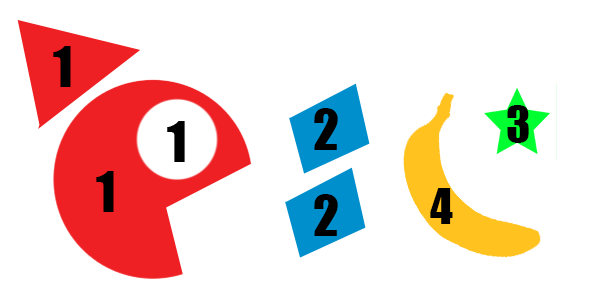
\includegraphics[width=\linewidth]{img/schemamergerA.png}
        \caption{Représentation des \texttt{Shapes} \{<1,1,1>,<2,2>,<3>,<4>\}}
    \end{subfigure}%
    ~ \\
    \begin{subfigure}{.7\linewidth}
        \centering
        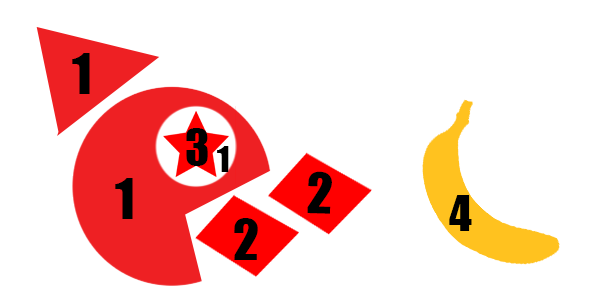
\includegraphics[width=\linewidth]{img/schemamergerB.png}
        \caption{Fusion des \texttt{Shapes} 1, 2 et 3}
    \end{subfigure}
    
    \caption{Fusion des groupes de \texttt{Shapes}: \{<1,1,1,2,3,3>,<4>\}}
    \label{fig:schemamerger}
\end{figure*}



Les deux classes Transformer et Merger ont été séparées car l'exécution du Merger est indépendante de celle du Transformer choisi. Cela permet également de simplement modifier la configuration de départ d'un algorithme en ne faisant aucun appel à Merger.


\paragraph{Solvers}

La classe \texttt{Solver} est également abstraite, elle contient les méthodes virtuelles \texttt{preSolve} et \texttt{solveBin} qui permettent respectivement d'effectuer le traitement préliminaire nécessaire au bon fonctionnement du \texttt{Solver} et d'appliquer l'algorithme de résolution sur une seule plaque (en utilisant un sous-ensemble des \texttt{Shapes}).
La méthode \texttt{solveBin} travaille sur une liste d'indices lui indiquant les formes qu'il reste à packer. Lorsqu'une forme est placée sur la plaque, son indice est retiré de la liste.


\subsubsection{Outer}

La dernière étape de l'exécution a pour objectif d'écrire un fichier SVG contenant toutes les formes sélectionnées par l'utilisateur, après leur traitement par la classe \texttt{Solver}. Ceci est réalisé par la classe \texttt{Outer}, qui, à partir des formes précédemment déplacées par le \texttt{Solver} et de leurs identifiants récupérés par la classe \texttt{Parser}, va recopier les éléments associés à ces identifiants sur la sortie standard. \\

On parcourt donc l'arborescence du fichier SVG, en utilisant \texttt{rapidXML}, de manière à sélectionner les éléments en fonction de leur identifiant, pour ensuite ajouter un champ contenant la matrice de transformation associée aux déplacements effectués lors du packing (ou de modifier si le champ existe déjà).

La représentation obtenue au format SVG est alors stockée sous forme de chaîne de caractères dans un attribut de l'instance associée. %seems better 

Dans le cas d'une duplication (en bas de page), tous les éléments de l'arborescence parsés lors du parcours sont d'abord recopiés sans être modifiés. 
Les formes sont ensuite regroupées par plaques, en utilisant leurs coordonnées.
Ces groupes sont ensuite écrits dans le format SVG sur la sortie standard qui sera récupérée par le plugin ou par l'utilisateur pour être écrite dans un fichier.


%SCHEMA OUTER ICI
\subsection{Langage de script}
Tous les algorithmes précédemment évoqués sont dans des classes. Cela signifie que pour exécuter certains algorithmes dans un certain ordre, il fallait à l'origine instancier chacune des classes et appeler les bonnes méthodes sur ces derniers, imposant de recompiler le projet pour tout changement dans cet ordre ou dans les paramètres passés aux algorithmes.\\

Le temps de compilation du projet étant tout sauf instantané, il nous est apparu qu'il était nécessaire d'avoir une solution permettant de définir cet ordre à l'exécution plutôt qu'à la compilation. Nous avons alors eu l'idée d'introduire un langage de script extrêmement minimaliste permettant simplement de définir un ordre d'exécution ainsi que de passer des paramètres aux algorithmes.\\

Plutôt que de réaliser un parser ad-hoc pour ce nouveau langage, nous avons préférer le définir sous la forme d'une grammaire, et se reposer sur le module \texttt{Qi} de la librairie \texttt{Boost Spirit}, qui permet de construire des parsers basés sur une grammaire définie entièrement en C++, ce qui permet d'éviter une étape supplémentaire du type \texttt{yacc}n grâce à une redéfinition habile de multiples opérateurs.\\

Nous voulions comme fonctionnalités de base l'appel d'un \texttt{Solver} ou d'un \texttt{Transformer} avec des paramètres potentiels, ainsi que la possibilité de répéter des blocs d'instructions. Nous sommes alors arrivé à la grammaire fournie en annexe.\\

On constate qu'une instruction est alors toujours de la forme
$$\texttt{Fonction(param1=valeur1, param2=valeur2, ...);}.$$
et qu'on peut faire des blocs de telles instructions avec les mots-clés \texttt{BEGIN} et \texttt{END}, puis repéter de tels blocks avec la syntaxe \texttt{DO <X> TIMES <bloc>}.\\

\begin{figure}[H]
\centering
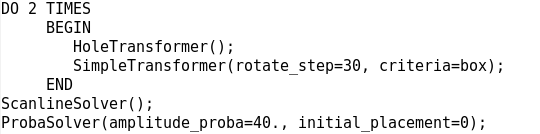
\includegraphics[scale=0.6]{img/closeEnough.png}
\caption{Un exemple de script}
\label{fig:closeEnough}
\end{figure}

On peut ainsi voir un exemple de script en figure~\ref{fig:closeEnough}. Dans ce dernier, on commence par exécuter \texttt{HoleTransformer}, puis \texttt{SimpleTransformer} (auquel on passe un entier et une chaîne de caractères), le tout deux fois. On appelle ensuite \texttt{ScanlineSolver} et \texttt{ProbaSolver}, auquel on passe un flottant et un entier.\\

À la manière de \texttt{yacc}, on associe à chaque règle un type et donc une valeur qui sera affectée à une instance de cette règle lors du parsing. On définit les actions grâce à une syntaxe spécifique à \texttt{Qi}. Nous avons choisi de stocker des informations basiques comme les noms, l'ordre, les paramètres des fonctions au fur et à mesure du parsing, et d'exécuter tout ce qui a été stocké à la fin de chaque \texttt{<big\_block>}.\\

Lors de l'exécution, il fallait associer à un nom de fonction dans le script une classe à instancier. Cela était au départ réalisé par une simple structure du type \texttt{if ... else if...}, mais quand le nombre d'algorithme a augmenté, nous avons voulu adopter une méthode plus générique.\\

Nous avons alors réalisé un mécanisme de registre, utilisant de manière intense la meta-programmation et les templates, permettant simplement d'instancier sur le tas une classe à partir de son nom et de lui transmettre les paramètres de l'utilisateur de façon entièrement automatique. Un registre est en fait un type disposant de méthodes statiques et se crée de la manière suivante :
$$\texttt{using NewReg = Registry<Base, boost::mpl::set<Derived1, Derived2, ...>::type>}$$

Les classes \texttt{Derived} devant hériter de \texttt{Base}. Toutes les classes doivent prendre en paramètre un ensemble de formes et un tableau de paramètres. Après la définition de ce nouveau registre, il faut initialiser sa table interne en appelant \texttt{NewRegistry::Init()} une unique fois. Il suffit ensuite pour instancier une classe depuis son nom d'appeler :
$$\texttt{NewReg::instanciate("Derived2", shapes, params)}$$
Cette fonction retourne un \texttt{Base*} contenant une instance de \texttt{Derived2}. De plus, les règles de la grammaire peuvent être écrites de manière automatique grâce à ce mécanisme (en exploitant le registre, qui contient en interne une \texttt{map} entre chaînes de caractère et pointeurs sur fonction).\\

Ainsi lorsqu'on veut ajouter un \texttt{Solver} ou un \texttt{Transformer} à la grammaire, il suffit seulement d'ajouter son type à la définition du registre, et tout le reste est généré automatiquement. Nous obtenons donc un langage de script très facile à étendre.\\

Pour exécuter nos algorithmes, il ne reste alors qu'à appeler le parser généré depuis le \texttt{main}, et tous les algorithmes sont exécutés au cours du parsing.
    


%--------------------------------------------------------
%	 ALGORITHMES

%--------------------------------------------------------
\section{Algorithmes}
%IV - Algorithmes transformers - presolveurs - solveurs
%    1. Transformers
%    1.1 Simple Transformer[dodo]
%    1.2 Hole Transformer[elodie]
%    
%    2. Solveurs et leur presolveurs
%    2.1 ToInfinityAndBeyond
%    2.2 TheSkyIsTheLimit
%    2.3 ScanLine
%    (2.4 Solveur physique)
%    (2.5 Solveur probabiliste)


%% Rappel : à ce moment du rapport, on a déjà expliqué l'architecture du code - PLEASE DO NOT REPEAT ;)

%% TRANSFORMERS
\subsection{Transformers}
La classe Transformer a pour but de regrouper plusieurs sous-ensembles de formes en 'blocs'. Ce sont des algorithmes appliqués sur les formes avant l'étape de packing, ils servent à augmenter l'efficacité globale du programme, en cherchant des formes à assembler ensemble selon différents critères : les formes d'un 'bloc' sont choisies de manière à ce que l'aire occupée par le bloc soit la plus faible possible.
Certains transformers utilisent plusieurs critères de qualité : aire d'intersection entre enveloppes convexes, taille de la bounding box résultante etc.

L'intérêt de la classe Transformer est de pouvoir proposer un packing plus optimal qu'un algorithme solveur, mais seulement de manière locale (temps d'exécution qualitativement excessif).

En fin de tâche, la classe Transformer envoie un ensemble d'informations à la classe Merger pour que celle-ci puisse modifier la représentation interne des formes afin que les algorithmes suivants considèrent effectivement les formes déplacées comme un bloc insécable.


\subsubsection{Simple Transformer}

\indent Le \texttt{Simple Transformer} est un algorithme de packing \textit{brute force} qui, pour deux formes données, teste un ensemble de dispositions entre elles pour optimiser un critère de l'union résultante.\\

Pour cela, on effectue une série de rotations de la première forme sur elle-même, d'un angle $\alpha$. Puis on effectue une autre série de rotations d'un angle $\beta$ sur la seconde forme de la même façon. Pour chaque couple de rotations, la seconde forme est ensuite déplacée de façon à être alignée avec la première forme, selon l'axe $x$. Un léger \textit{offset} selon l'axe $y$ est ajouté pour tester toutes les configurations possibles (à la précision de l'\textit{offset} et des angles près). 

On minimise la distance entre les deux formes en translatant la deuxième selon l'axe des $x$, jusqu'à ce que les deux pièces se touchent, le tout par dichotomie. Tout le procédé est illustré en figure~\ref{fig:simpletransformer}.\\

On garde finalement le triplet $(\alpha, \beta, offset)$ minimisant un certain critère, passé en paramètre. Nous avons par exemple la minimisation de la bounding box résultante (utile lorsqu'on va utiliser un algorithme sur rectangles ensuite) ou bien la maximisation de l'aire d'intersection entre les enveloppes convexes.


\begin{figure}[!htb]
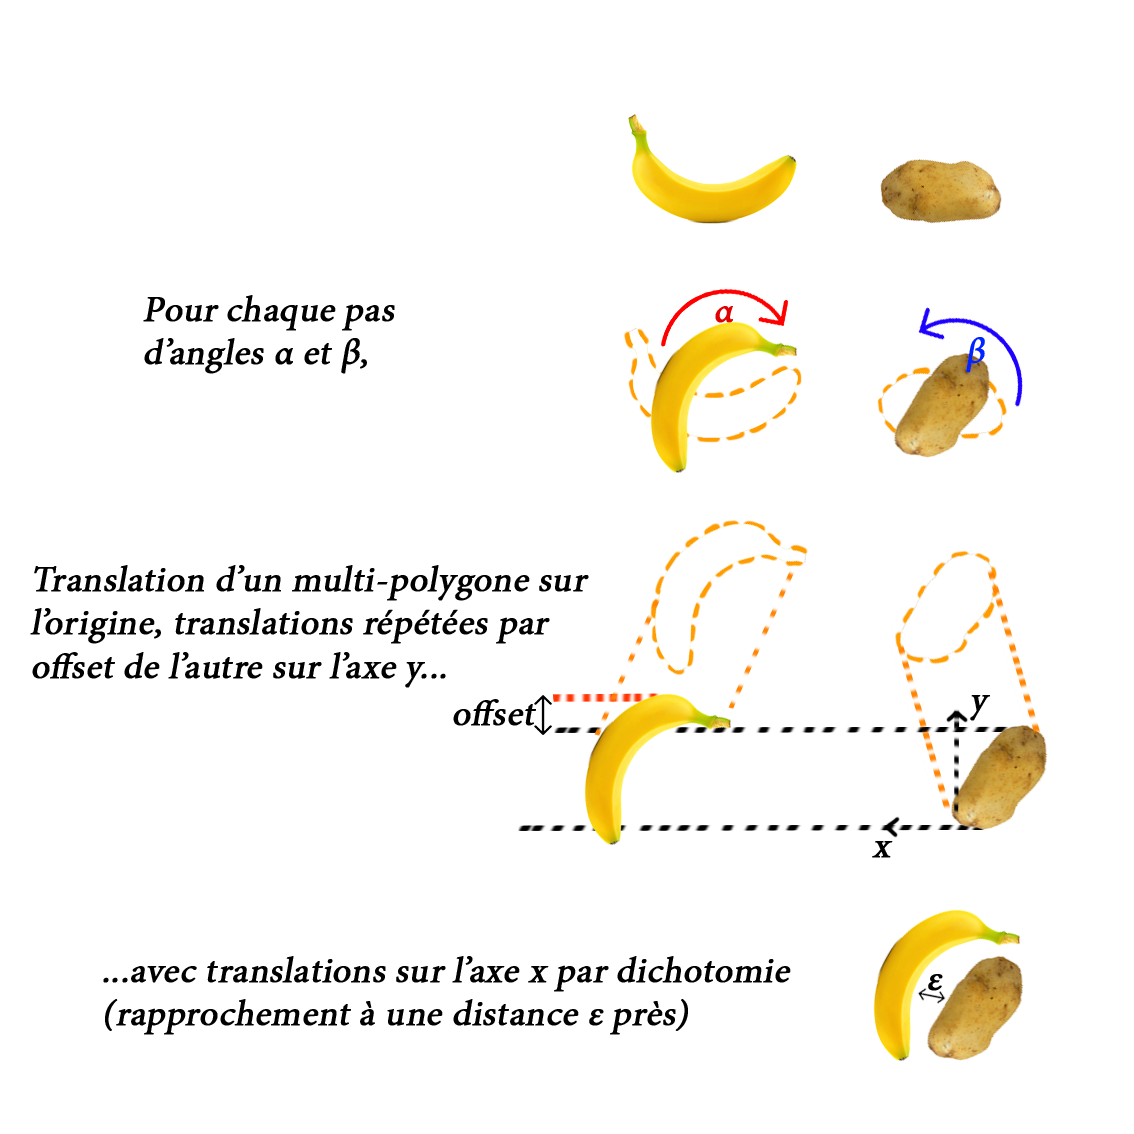
\includegraphics[scale=0.4]{img/simpletransformer.png}
\caption{Illustration du procédé de \texttt{SimpleTransformer}}
\label{fig:simpletransformer}
\end{figure}
%banana for scale

\subsubsection{Hole Transformer}
Le but de cet algorithme est de remplir les trous de formes trouées avec d'autres pièces de l'ensemble de Shapes. Cette étape peut s'avérer utile car dans les solveurs employés par la suite, on utilise au mieux les enveloppes extérieures des formes, sinon leur bounding box, empêchant ainsi toute pièce de jamais combler les trous d'une autre. 

Le pseudo-algorithme \ref{alg:hole} ci-dessous décrit le fonctionnement de ce transformer.

\begin{algorithm}
    \caption{- Hole Transformer}
    \label{alg:hole}   
    \textbf{Entrée} : Ensemble de formes\\
    \textbf{Sortie} : Vecteur de n-uplets des indices de formes à fusionner, avec leur nouvelle position\\

    \textbf{Début}\\
    \hspace{0.5cm}Établir une liste des trous triés par ordre décroissant d'aire;\\
    \hspace{0.5cm}Trier les formes par ordre croissant d'aire;\\
    \hspace{0.5cm}\textbf{Pour chaque} trou t :\\
        \hspace{1cm}\textbf{Pour chaque} forme f :\\
        \hspace{1cm}\textbf{Si} aire(f) < aire(t) \textbf{et} f n'a pas déjà été choisie:\\
            \hspace{1.5cm}Déplacer f au centre de t; //centre f = centre t \\
            \hspace{1.5cm}\textbf{Si} pas de collision entre f et t :\\
                    \hspace{2cm}Ajouter (f,t) au vecteur de sortie ; \\
                    \hspace{2cm}Marquer f comme déjà choisie ;\\
    \hspace{0.5cm}\textbf{Retourner} le vecteur de tuples;\\
    \textbf{Fin}\\
\end{algorithm}

Cet algorithme est assez simple, il ne place au mieux qu'une seule forme par trou - en son centre, et n'effectue pas de rotation pour une meilleure recherche de compatibilité.



%%SOLVERS
\subsection{Solvers}

\subsubsection{Algorithmes par \textit{bounding box}}

Trois algorithmes ont été implémentés en utilisant des boîtes englobantes rectangulaires englobant les différentes formes : le problème est alors ramené à un packing de rectangles, beaucoup plus simple (mais qui reste \textit{NP-complet}).\\

\begin{figure}[!htb]
\centering
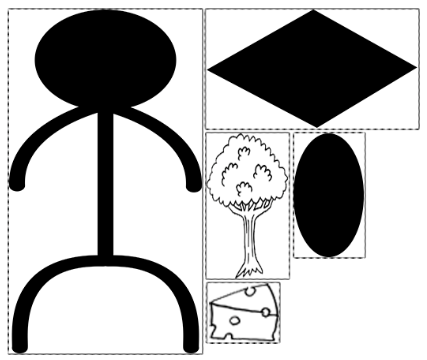
\includegraphics[scale=0.7]{img/boundingBox.png}
\caption{Illustration du procédé des bounding boxes}
\label{fig:boundingBox}
\end{figure}

\indent Les deux premiers solveurs, \texttt{LineSolver} et \texttt{MultilineSolver} sont des plus basiques, mais ils permettent au moins de disposer les pièces sur les plaques sans intersection. L'algorithme \texttt{ScanLineSolver} est plus complexe et fournit une bien meilleure compacité.\\

L'algorithme \texttt{LineSolver} se contente d'aligner les formes de façon désordonnée sur une ligne, sans retour lorsque l'on dépasse la taille de la plaque. Pour cela il colle les rectangles entre eux au plus proche. Lorsque la largeur de la plaque est dépassée, il passe à une plaque suivante.\\

L'algorithme \texttt{MultilineSolver} en est une version améliorée. Les différentes boîtes sont triées par hauteur et sont placées par hauteurs décroissantes.
Le packing va alors se faire ligne par ligne, en insérant les pièces depuis le bord gauche jusqu'à atteindre le bord droit de la plaque. Les lignes sont ensuite juxtaposées les unes en dessous des autres. Un exemple de sortie peut être constaté en figure~\ref{fig:multilineSolver}.

\begin{figure}[!htb]
\centering
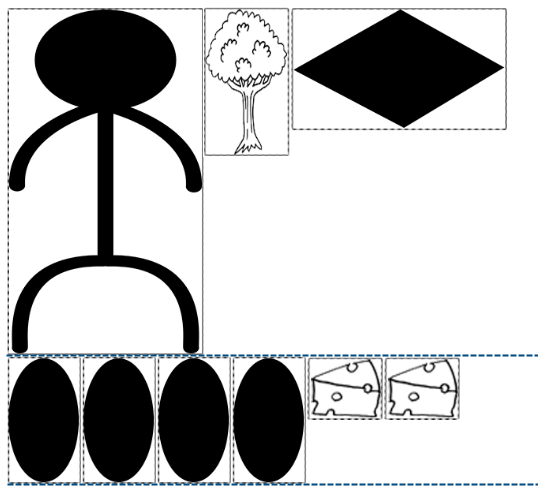
\includegraphics[scale=0.6]{img/multilineSolver.png}
\caption{Exemple d'une sortie du \texttt{MultilineSolver}}
\label{fig:multilineSolver}
\end{figure}

Le solveur \texttt{ScanLine} utilise l'algorithme connu du \textit{first-fit}. Il commence par affiner la boîte englobante au mieux : des rotations sont effectuées sur les pièces afin d'obtenir la boîte avec un rapport (aire vide / aire boîte) le plus faible. Ces boîtes sont ensuite triées par ordre décroissant de hauteur, comme l'illustrent la figure~\ref{fig:ScanlineA}.

\begin{figure}[!htb]
\centering
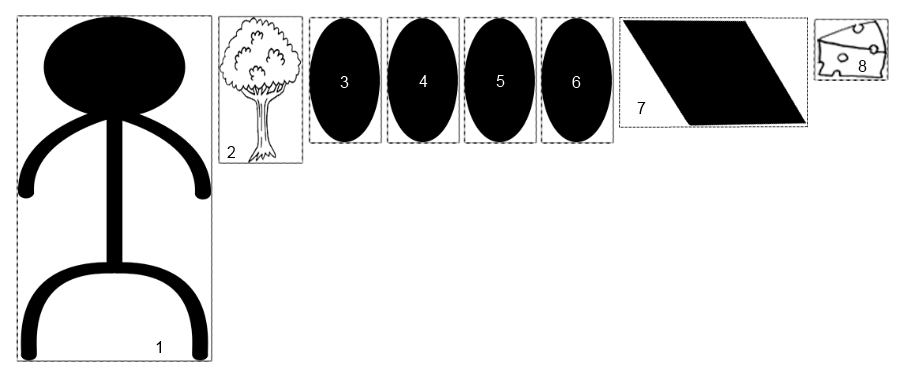
\includegraphics[scale=0.6]{img/ScanlineA.png}
\caption{Jeu de pièces, affinées à la meilleure bounding box, puis triées}
\label{fig:ScanlineA}
\end{figure}

\newpage
\indent L'essentiel du packing va consister à manipuler une grille de cellules rectangulaires dans l'état "plein" ou "vide", et de déterminer un ensemble de cellules dans lequel une boîte peut rentrer. Le parcours de cette grille s'effectue colonne par colonne de haut en bas, de gauche à droite. Dès qu'une place est trouvée pour la boîte, c'est-à-dire un ensemble de cellules toutes vides, la grille est mise à jour pour correspondre exactement aux nouvelles cellules pleines et vides avec les boîtes placées (figure~\ref{fig:ScanlineC2-3}).

\begin{figure}[!htb]
\centering
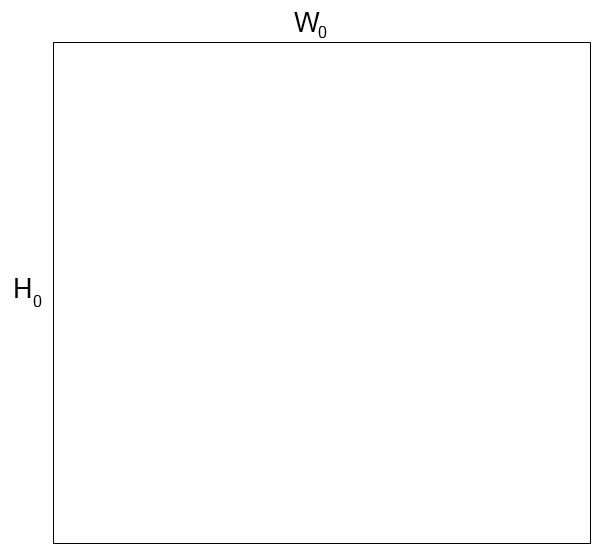
\includegraphics[scale=0.4]{img/ScanlineC1.png}
\caption{La plaque initiale est une grille à une seule cellule vide}
\label{fig:ScanlineC1}
\end{figure}

\begin{figure*}[!htb]
    \centering
    \begin{subfigure}{.48\linewidth}
        \centering
        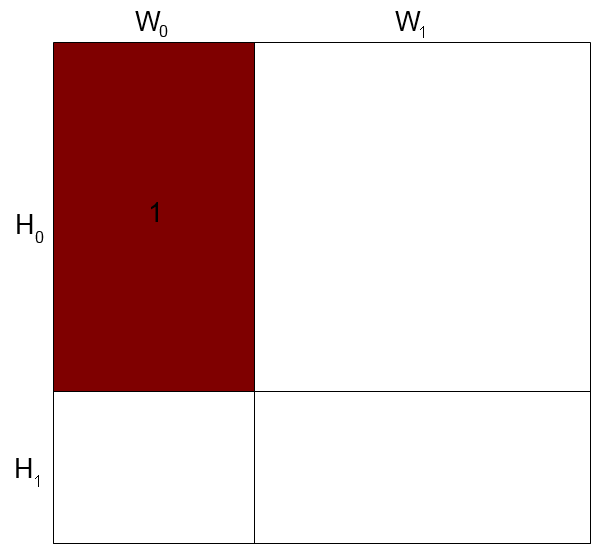
\includegraphics[width=\linewidth]{img/ScanlineC2.png}
        \caption{Ajout de la pièce 1 en $(W_0,H_0)$}
    \end{subfigure}%
    ~ 
    \begin{subfigure}{.48\linewidth}
        \centering
        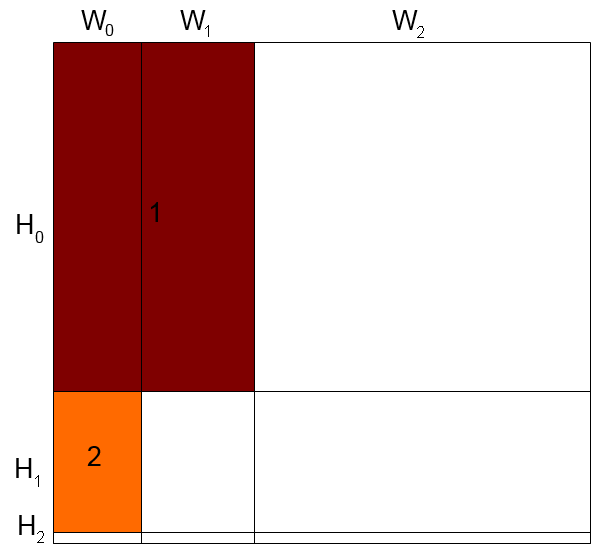
\includegraphics[width=\linewidth]{img/ScanlineC3.png}
        \caption{Ajout de la pièce 2 en $(W_0,H_1)$}
    \end{subfigure}
    \caption{A chaque ajout de pièce, la grille est redécoupée}
    \label{fig:ScanlineC2-3}
\end{figure*}

\begin{figure*}[!htb]
    \centering
    \begin{subfigure}{.48\linewidth}
        \centering
        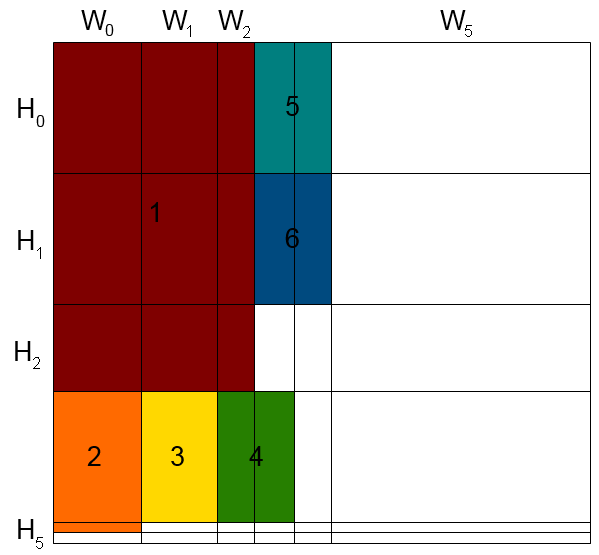
\includegraphics[width=\linewidth]{img/ScanlineC4.png}
        \caption{Grille après insertions des pièces 1 à 6}
    \end{subfigure}%
    ~ 
    \begin{subfigure}{.48\linewidth}
        \centering
        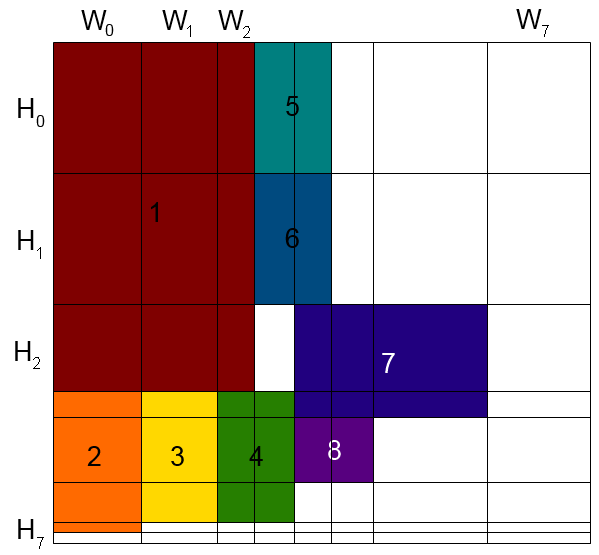
\includegraphics[width=\linewidth]{img/ScanlineC5.png}
        \caption{Les insertions peuvent créer des trous}
    \end{subfigure}
    \caption{Une pièce s'insère le plus à gauche, puis le plus en haut possible}
    \label{fig:ScanlineC4-5}
\end{figure*}

\begin{figure}[!htb]
\centering
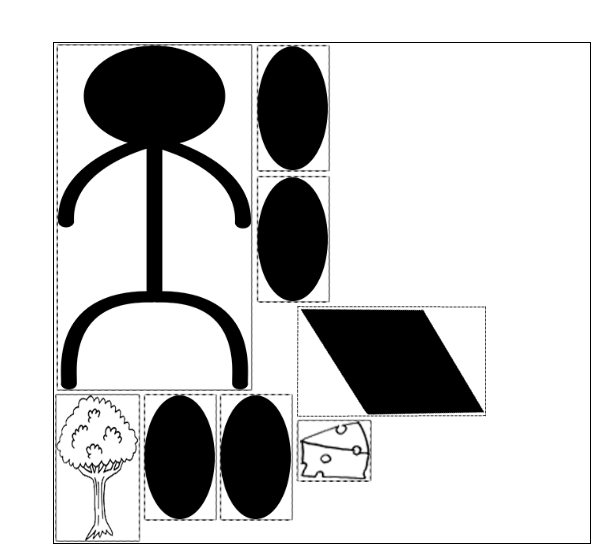
\includegraphics[scale=0.5]{img/ScanlineC6.png}
\caption{Sortie de l'algorithme \texttt{ScanlineSolver}}
\label{fig:ScanlineC6}
\end{figure}

\newpage
\indent Il se peut que la succession des insertions et la maximisation de la compacité laisse une cellule vide entre les pièces, les plus grandes ne pouvant pas s'y placer (figure~\ref{fig:ScanlineC4-5}). Toutefois les pièces sont triées par ordre décroissant de hauteur, aussi les pièces les plus petites combleront ces cellules vides pour améliorer davantage la compacité de la plaque finale.

\newpage
Enfin, une dernière optimisation est effectuée une fois que toutes les pièces ont tenté une insertion: ces pièces sont tournées de 90°, puis un nouvel essai d'insertion. Cela conserve les propriétés rectangulaires dont le solver a besoin, et une pièce plus large que longue peut donc rentrer dans un ensemble de cellules jusque-là trop petit.

\begin{figure}[!htb]
\centering

\includegraphics[scale=0.5]{img/ScanlineClounk.png}
\caption{Une pièce trop large peut être insérée après rotation}
\label{fig:ScanlineClounk}
\end{figure}


\subsubsection{Algorithmes non déterministes}

Les autres algorithmes implémentés insèrent les pièces de manière partiellement aléatoire sur la plaque.\\

\paragraph{FreezeSolver}
Le solver \texttt{FreezeSolver} assimile la plaque à un panier que l'on remplit, et fait tomber les pièces une à une dans la plaque grâce à de petites translations qui simulent la gravité pendant un certain nombre d'itérations.\\
\indent La pièce tombe alors vers le bas de la plaque et en cas de collision avec les bords ou le fond, la pièce est repoussée vers l'intérieur. Après un certain temps de calcul, le solver vérifie que la position de la pièce est valide (c'est-à-dire entièrement dans la plaque, et sans collision générée par les dernières translations-rotations), la pièce se fige et la suivante est lâchée à partir du haut (figure~\ref{fig:FreezeAB}).\\

\begin{figure*}[!htb]
    \centering
    \begin{subfigure}{.4\linewidth}
        \centering
        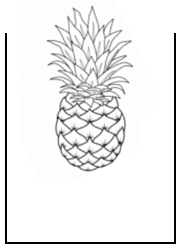
\includegraphics[width=\linewidth]{img/FreezeA.png}
        \caption{La pièce 1 est lachée du haut de la plaque}
    \end{subfigure}%
    ~ 
    \begin{subfigure}{.4\linewidth}
        \centering
        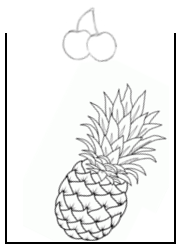
\includegraphics[width=\linewidth]{img/FreezeB.png}
        \caption{La pièce 1 se fige, et la pièce 2 est lachée}
    \end{subfigure}
    \caption{Le \texttt{FreezeSolver} s'apparente à un panier}
    \label{fig:FreezeAB}
\end{figure*}


Si une pièce entre entre collision avec une autre lors du calcul, alors elle est expulsée vers le haut, translatée aléatoirement à gauche ou à droite, et pivotée aléatoirement dans un sens ou dans l'autre avant de recommencer à tomber, ce qui simule un entassement des pièces dans la plaque (figure~\ref{fig:FreezeCD}).\\

\begin{figure*}[!htb]
    \centering
    \begin{subfigure}{.30\linewidth}
        \centering
        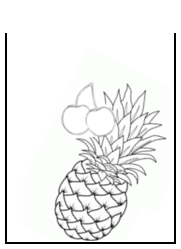
\includegraphics[width=\linewidth]{img/FreezeC.png}
    \end{subfigure}%
    ~ 
    \begin{subfigure}{.30\linewidth}
        \centering
        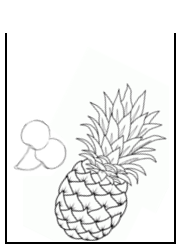
\includegraphics[width=\linewidth]{img/FreezeD.png}
    \end{subfigure}
    ~ 
    \begin{subfigure}{.30\linewidth}
        \centering
        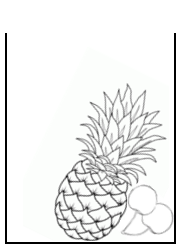
\includegraphics[width=\linewidth]{img/FreezeE.png}
    \end{subfigure}
    
    \caption{Lors d'une collision, la pièce est repoussée à gauche ou à droite}
    \label{fig:FreezeCD}
\end{figure*}

De plus, si le solver n'arrive pas à stabiliser la pièce, c'est-à-dire si elle est toujours en collision avec une autre après de multiples essais de corrections, celle-ci est envoyée vers une seconde plaque pour être packée. Cela se produit naturellement lorsque la plaque est déjà saturée et ''déborde''.

\begin{figure}[!htb]
\centering
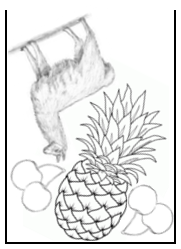
\includegraphics[scale=1]{img/FreezeG.png}
\caption{Sortie de l'algorithme \texttt{FreezeSolver}}
\label{fig:FreezeSolver}
\end{figure}

\paragraph{ProbaSolver}
Notre deuxième algorithme "non déterministe" est ce que nous avons appelé le \texttt{ProbaSolver}. Il s'agit cette fois-ci d'un solveur entièrement basé sur l'aléatoire. Le principe de base est le suivant : en partant d'une configuration sans intersection des pièces, on effectue pour chaque pièce une translation et une rotation aléatoire. L'amplitude de ces mouvements dépend d'une distribution exponentielle, de la forme $\lambda e^{-\lambda t}$, avec $\lambda$ passé en paramètre du solveur. Cette distribution permet d'obtenir la plupart du temps des mouvements de faible amplitude (d'autant plus que $\lambda$ est grand), sans pour autant exclure des mouvements importants permettant d'explorer plus de configurations.\\

Pour chaque pièce, on vérifie une fois ce mouvement effectué qu'elle ne touche aucune autre pièce et ne sort pas de sa plaque, autrement le mouvement est inversé. Seule exception : si la pièce sort de la plaque par le haut, on lui offre une opportunité de gravir les échelons (monter d'une plaque).\\

On effectue ces pas aléatoires pendant un nombre fixé d'itération, après quoi on s'arrête et on évalue la qualité de la solution. On sauvegarde cette solution et sa qualité (sous la forme d'un tableau de matrices de transformations), et on recommence le procédé entièrement. À la fin de celui-ci, on regarde si la solution obtenue est meilleure que la solution sauvegardée, auquel cas remplace la sauvegarde (sinon, on restaure l'ancienne solution).\\

On répète encore ce procédé d'amélioration un certain nombre de fois, jusqu'à arriver à une solution normalement satisfaisante, avec de la chance.

% Quelques chiffres:

% Multiline :
% Scanline :
% Freeze :
% Proba :


%--------------------------------------------------------
%	 OPTIMISATION
%--------------------------------------------------------
\section{Optimisation}
\subsection{Quad-Tree}

Nous avons implémenté une autre manière de considérer les formes lors du packing en utilisant une structure de donnée particulière : les \texttt{quadtrees}.

\subsubsection{Principe général}

Prenons la bounding box d'un multi polygone. On le représente par une matrice de 0 et de 1 (bitmap). L'algorithme de création du quadtree consiste en subdivisions successives de la bounding box en zones. On délimite la bounding box de départ en 4 parties de tailles égales, puis on délimite ces zones en 4 parties récursivement, jusqu'à arrivée à un stade terminal.

A chaque itération, on regarde si une partie du multi polygone est contenue dans la zone en cours. Si non, on considère la zone comme "blanche" (0) et la récursivité se termine sur cette zone. Si le multi polygone recouvre intégralement la zone en cours, on considère cette dernière comme "noire" (1) et la récursivité se termine également. Le stade terminal peut également être une zone de taille atomique (pixel), une zone de précision voulue. 

Si le multi polygone est en partie dans la zone en cours, il s'agit d'une zone dite "grise", c'est-à-dire que la précision de la zone n'est pas suffisante pour décrire suffisamment le multi polygone sous forme de quadtree. Dans ce cas-ci, la subdivision récursive a lieu. Quelques itérations sont représentées en figure ~\ref{fig:quadtreeprinciple}.

\begin{figure}[H]
\centering
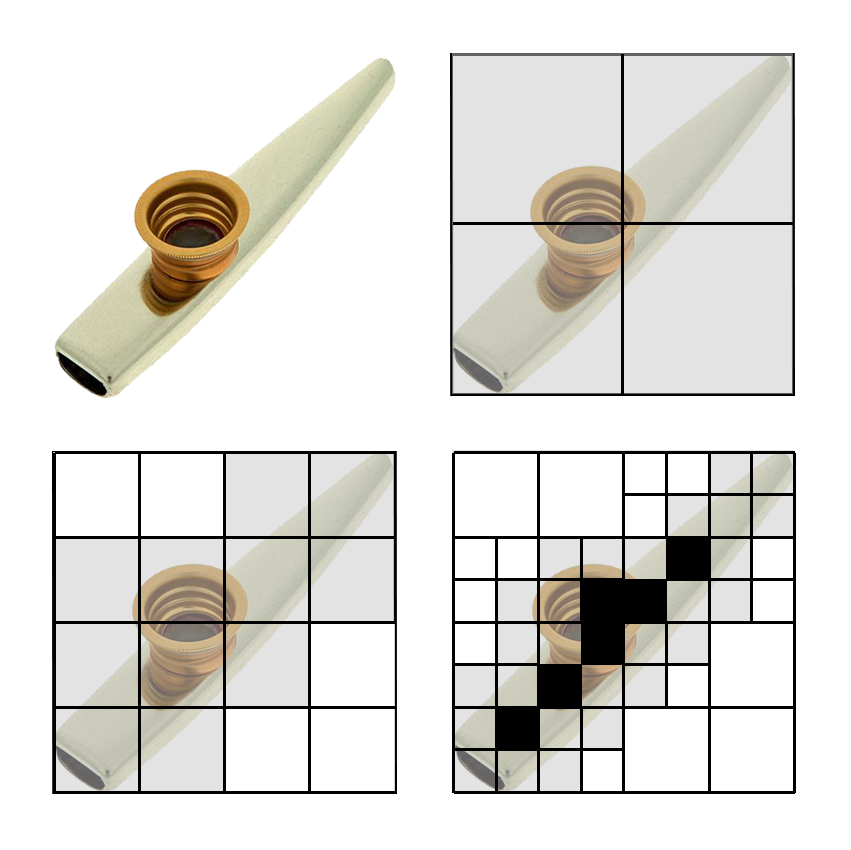
\includegraphics[scale=0.5]{img/quadtreeprinciple.png}
\caption{Principe du quadtree, itérations 0 à 3.}
    \label{fig:quadtreeprinciple}
\end{figure}

\subsubsection{Représentation}

Un Quadtree est une classe de même nom contenant plusieurs InnerQuadTree avec plusieurs informations sur ces derniers pour les utiliser par la suite. Plus clairement, on a choisi de précalculer pour un même multi polygone plusieurs quadtrees pour un ensemble de rotations possibles (30 degrés par défaut, donc 12 quadtrees précalculés). La classe Quadtree les garde en mémoire, ainsi que les offsets nécessaires (pour gérer la différence de point d'origine entre un multi polygone (au centre) et un quadtree(en haut à gauche)), les centres de gravité de chaque rotation (centroids) et d'autres informations (précision de l'approximation etc).\\


Les InnerQuadTrees s'occupent de la récursivité en elle-même. La classe contient la couleur de la zone, sa profondeur par rapport à la racine, sa bounding box, sa taille et les 4 InnerQuadTree éventuels (sous-espaces) à la profondeur suivante (voir figure ~\ref{fig:innerquadtree}.

\begin{figure}[H]
\centering
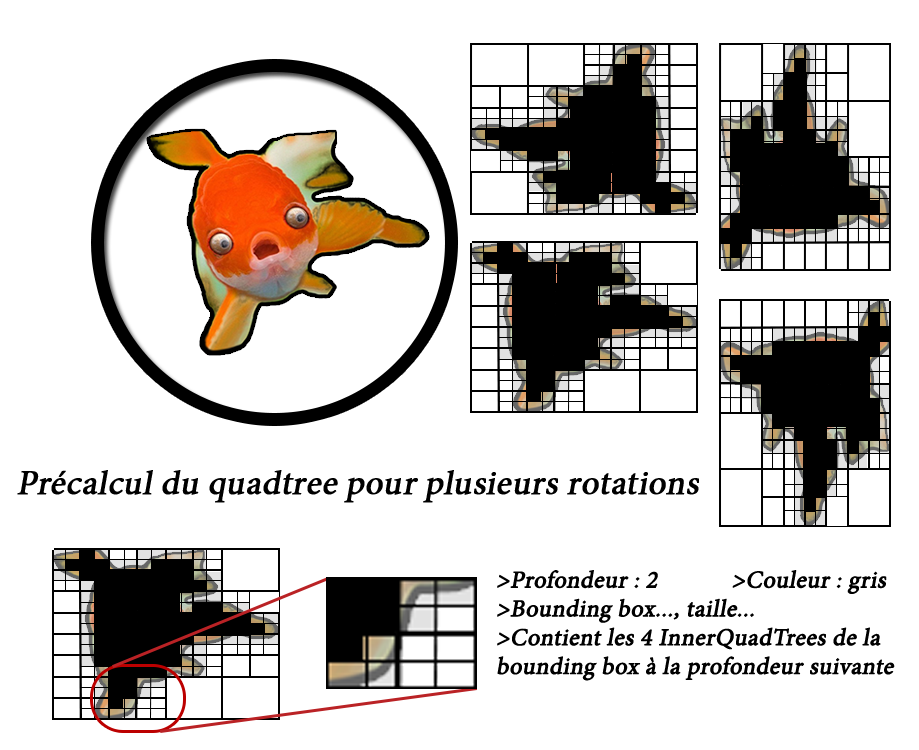
\includegraphics[scale=0.5]{img/innerquadtree.png}
\caption{Les InnerQuadTrees et leurs informations}
    \label{fig:innerquadtree}
\end{figure}

Pour tester la couleur de son espace et créer les sous-espaces suivants, un InnerQuadTree possède des méthodes appelant celles des bitmaps, représentés également par une classe. Un bitmap est une classe représentant un tableau de booléens qui est le même pour toutes les classes (utilisation d'un pointeur), avec les informations nécessaires pour situer la sous-zone concernée dans l'espace (offsets, taille...). La classe bitmap possède les méthodes primaires d'intersection, de translation, de rotation, de création etc.


\subsection{Parallélisme}

Une autre possibilité pour améliorer l'efficacité générale du programme est d'exploiter les architectures multicoeur qui sont disponibles sur les machines récentes. Nous avons utilisé cette notion de parallélisme de deux façons:\\

\subsubsection{Parallélisation d'un algorithme} Au cours du projet, nous avons développé plusieurs solutions. Certaines d'entre elles effectuant un grand nombre d'opérations indépendantes (notamment le \texttt{Simple Transformer}), il est possible de répartir le calcul de ces opérations sur plusieurs processeurs afin d'accélérer l'exécution du programme. 

\subsubsection{Parallélisation de plusieurs algorithmes} Certains algorithmes ayant un comportement non déterministe, plusieurs exécutions d'un même algorithme vont conduire à des résultats différents.
Nous avons donc implémenté un \texttt{Solver} permettant d'effectuer plusieurs calculs de solutions non déterministes et de conserver seulement le meilleur résultat.


\subsection{Interpolation améliorée}

Dans le but d'améliorer la vitesse d'exécution des algorithmes nous avons mis en place une méthode d'interpolation visant à réduire au maximum le nombre de points, tout en minimisant l'erreur induite.\\ 

Ceci permet d'effectuer plus rapidement les calculs internes aux algorithmes fonctionnant directement sur les modèles basés sur les points (\texttt{Shape}) en plus de permettre un calcul plus rapide des \texttt{QuadTrees}.\\

Nous utilisons pour cela différentes propriétés des courbes de Bézier. Notamment le fait qu'une courbe de Bézier définie sur un intervalle restreint reste une courbe de Bézier, il est donc possible de découper récursivement les courbes et ce sans perte de précision.\\

Il a ensuite été nécessaire de déterminer une condition d'arrêt pour cet algorithme. Il nous a semblé naturel d'approximer la courbe par une droite lorsque celle-ci est suffisamment "plate".\\ Nous avons donc choisi d'approximer l'erreur générée par cette approximation par le maximum des distances des points de la courbe à la droite. \\%% MEH

Ceci permet en effet d'avoir une approximation relativement précise de l'écart minimal qu'il est possible de se permettre en représentation interne afin d'éviter les intersections en sortie. \\%% endMEH
Nous n'avons cependant pas été en mesure de calculer un majorant exact de l'erreur due à cette approximation. \\

\begin{figure}[!htb]
\centering
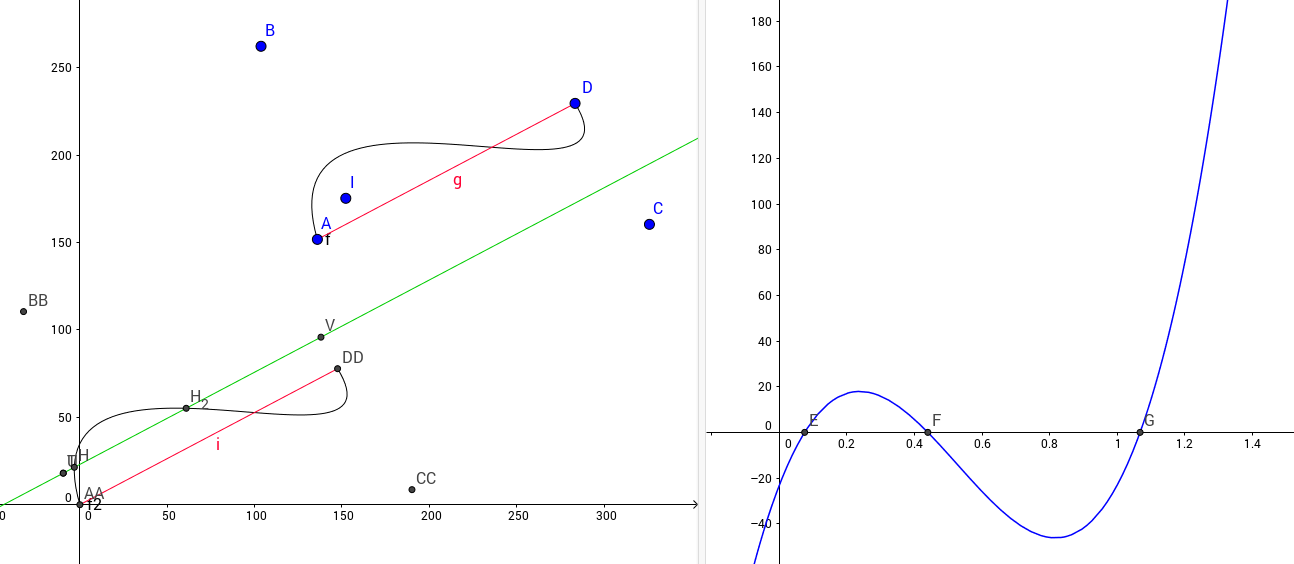
\includegraphics[scale=0.35]{img/BEZER.png}
\caption{Illustration de la recherche d'intersection}
\label{fig:rotos}
\end{figure}

Pour effectuer le calcul de cette distance maximale, nous calculons quatre points définissant les deux droites parallèles à celle définie par les deux points de contrôle de la courbe, qui se trouvent à une distance $d$ de celle-ci.\\

Nous utilisons ensuite la représentation paramétrique de ces droites, et de la courbe pour calculer s'il y a ou non intersection avec la courbe en résolvant une équation polynomiale du troisième degré sur l'intervalle $[0,1]$. Puis nous déterminons par dichotomie la distance $d$ maximale pour laquelle il y a intersection avec la courbe.\\

On peut voir sur la figure~\ref{fig:rotos} un exemple de droite s'intersectant avec une courbe de Bézier, et le polynôme associé.\\

Afin de compenser l'erreur ainsi produite, nous appliquons ensuite un \textit{buffer} autour de la forme définie par ces points, qui permet d'assurer que les bords de la nouvelle forme se trouvent à une distance égale à au moins deux fois l'erreur autorisée par l'approximation.\\

La marge d'erreur est réglable à la compilation, et une plus grande marge implique un \textit{buffer} plus important. On peut constater en figure~\ref{fig:rotos2} un exemple d'approximation très exagéré, avec le \textit{buffer} ajouté.

\begin{figure}[!htb]
\centering
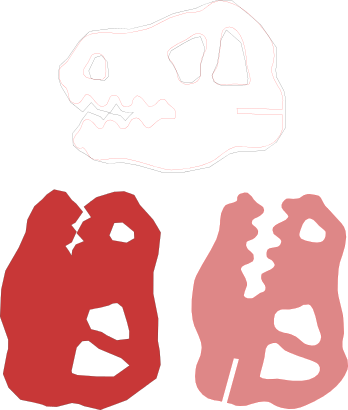
\includegraphics[scale=1.2]{img/approx.png} %non
\caption{Approximation (exagérée) d'une forme}
\label{fig:rotos2}
\end{figure}

\newpage
\section*{Conclusion}

%Bilan, a-t'on bien répondu aux attentes du client ? Que resterait-il à faire ? Que pourrait-on améliorer ? Quels futurs besoins à partir de cet outil ? 
Ainsi, le client a maintenant à sa disposition un ensemble d'outils pour le packing d'images vectorielles, utilisable sous Inkscape. Il peut facilement changer l'ordonnancement des solveurs grâce à un langage simple d'utilisation, changer la manière dont les objets vont être représentés lors des calculs, et ajouter de nouveaux algorithmes grâce à l'approche en programmation orientée objet.\\


On peut envisager de nombreux algorithmes pouvant s'ajouter à ceux implémentés. Par exemple, à la place d'utiliser des bounding boxes rectangulaires (Scanline), on pourrait affiner le packing avec d'autres formes comme des octogones, ou encore faire un solveur "physique", c'est-à-dire gérant les pièces comme des objets possédant un poids, dans une simulation de pesanteur, en les "remuant" d'une manière efficace pour parvenir à une solution assez stable. Encore une fois, c'est un problème NP-Complet, toute piste est intéressante dans une certaine mesure.\\

Dans le cadre de l'utilisation de la découpeuse laser, on peut également envisager une partie de code en amont s'occupant de définir les zones de packing relativement à la plaque réelle. Plus précisément, il s'agirait de construire par traitement d'image la plaque dans laquelle il faut packer les formes, selon présence de découpes déjà effectuées dedans ou non (utilisation éventuelle d'une webcam ?). Cela permettrait de récupérer au maximum les chutes de matériaux, et de mettre à profit nos solveurs sur plusieurs utilisations consécutives.\\


%--------------------------------------------------------
%	 Webographie
%--------------------------------------------------------
\newpage
\newpage

\section{Liens}

\textbf{Site du client (Eirlab) :}\\
    \url{http://www.eirlab.org/}
    
\textbf{Page commerciale de la machine laser :}\\
    \url{https://www.troteclaser.com/fr/machines-laser/machines-gravure-laser-speedy/}
    
    \href{https://www.troteclaser.com/fileadmin/content/images/Laser_Machines/Speedy_Series/Documentation-famille-Speedy.pdf}{Documentation technique de la machine}
    
\textbf{Bibliothèques utilisées :}\\
 \url{http://www.boost.org/}\\
 \url{http://svgpp.org/}\\
 \url{http://rapidxml.sourceforge.net/}\\

%%% PARTIE 5 : Architecture et Algorithmes

Plug-in mis à part, l'exécutable est organisé autour de trois modules principaux : \texttt{Parser}, \texttt{Solver} et \texttt{Outer}, qui servent respectivement à convertir un fichier SVG en notre représentation interne, à traiter cette représentation et à effectuer la conversion inverse, la classe \texttt{Solver} étant abstraite (elle implémente le packer identité) et permettant la création de "sous-solveurs" par héritage.\\

Les modules communiquent entre eux comme indiqué en figure~\ref{ps}.

\begin{figure}[hbt!]
\center
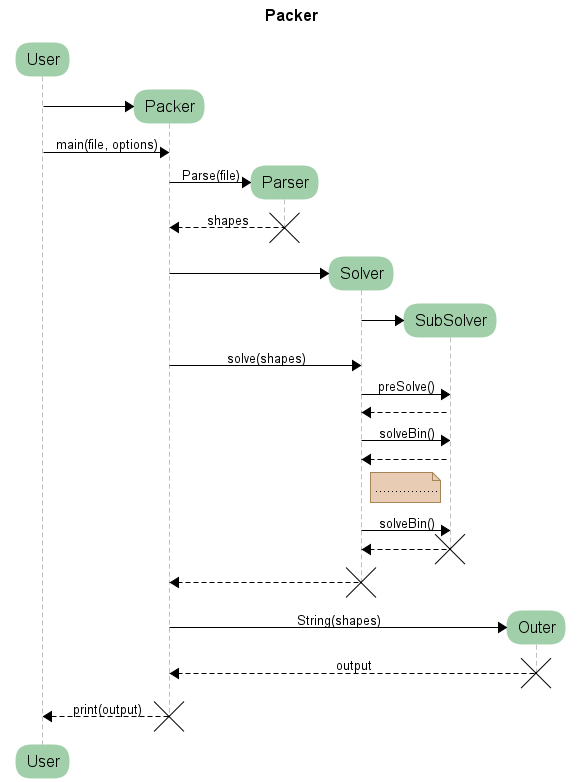
\includegraphics[scale=0.7]{img/packerSeq}
\caption{Diagramme de séquences du cas d'utilisation nominal}
\label{ps}
\end{figure}
\newpage
\subsection{Parser}

\texttt{SVG++} est utilisé comme aide au parsing : à l'aide de \texttt{rapidXML}, le fichier contenant les formes est lu sous forme d'arbre xml, puis il passe les informations qu'il parse à notre programme. Le nom des méthodes pour recevoir les informations de parsing est prédéfini, le code de chacune d'entre elle est alors à définir dans notre classe de \texttt{parseur} : il faut définir pour chaque type de balise SVG les actions à réaliser à l'entrée sur celles-ci (et potentiellement à la sortie) et les informations à stocker pour effectivement parser notre document.\\

\indent Les informations que nous cherchons à acquérir sont tout principalement les formes à packer, cependant nous avons également besoin de stocker d'avantage d'information pour effectuer un packing efficace, notamment les dimensions du document qui correspondent dans le cas ou cette information n'est pas passée en paramètre à la taille de la plaque sur laquelle réaliser le traitement.\\

\indent D'autres contraintes de fidélité nous poussent à gérer séparément d'autres informations telles que les matrices de transformation déjà présentes dans le fichier, et les groupes correspondant à des ensembles de pièces atomiques (par exemple une pièce trouée).\\


\indent Le dernier problème à s'être posé lors de la lecture du fichier est la présence de matrices de transformations dans les attributs des objets, des objets englobant plusieurs pièces tels que les groupes pouvant posséder de tels attributs, nous avons choisi d'utiliser une pile de matrices pour stocker la transformation à appliquer à l'élément actuel, cette transformation est égale au produit des différentes matrices à appliquer. On applique ensuite après l'interpolation la transformation aux points précédemment obtenus.

Un exemple d'exécution du parser est visible sur la figure~\ref{la pomme de terre} et recense la plupart des étapes effectuées au cours de celle-ci.

\begin{figure}[htb!]
\center
\hspace*{-2.2cm}
\includegraphics[scale=0.5]{img/ParserDiagram}
\caption{Exemple d'exécution du parser sur un arbre XML}
\label{la pomme de terre}
\end{figure}
\newpage

\subsection{Solver}

La classe \texttt{Solver} est la classe la plus importante de ce programme. Elle est destinée à accueillir les différents algorithmes de packing, par héritage. La classe de base implémente un solveur "identité", ainsi qu'un certain nombre de mécanismes utiles aux vrais solveurs qui en hériteront.\\
Son attribut principal est une référence sur un tableau de \texttt{Shape}, c'est à dire les formes à packer. Un solveur est censé avoir pour seul effet de modifier le tableau de \texttt{Shape} (c'est un effet de bord).\\

Pour implémenter un nouveau solveur, on peut redéfinir une ou deux méthodes de \texttt{Solver} : \begin{itemize}
    \item \texttt{preSolve}, qui permet au solveur d'effectuer des calculs préliminaires avant le packing lui-même (typiquement, un tri des formes),
    \item  \texttt{solveBin}, qui doit packer suffisamment de formes pour remplir une plaque, et sera appelée tant qu'il reste des formes à packer.\\
\end{itemize}

Pour signaler quelles formes restent à packer, on dispose dans la classe d'une liste (chaînée) d'indices sur le tableau de formes. Pour indiquer qu'une forme a été packée, le solveur doit retirer son indice correspondant dans la liste, et le packing s'arrête lorsque cette liste est vide.\\

Nous avons pour l'instant implémenté (en dehors du solveur identité) 3 solveurs différents (leur relation avec la classe mère est en figure~\ref{fig:uml}), qui respectivement mettent les formes triées sur une seule ligne, les mettent sur plusieurs lignes de manière à ce qu'on ne sorte pas de la plaque, et appliquent l'algorithme dit du "first-fit", qui est un algorithme efficace pour le packing de rectangles (il consiste à trier les formes puis à les insérer une par une sur la plaque le plus tôt possible. Il existe un ordre des formes pour lequel cet algorithme est optimal sur des rectangles).\\

\begin{figure}[htb!]
\center
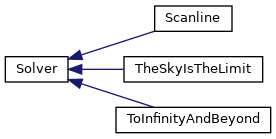
\includegraphics[scale=0.7]{img/solver_UML}
\caption{Diagramme UML de \texttt{Solver} et ses filles}
\label{fig:uml}
\end{figure}

Ces trois solveurs reposent d'ailleurs sur des rectangles enveloppant nos formes de bases, de manière à ne considérer que des rectangles lors du packing (ils sont donc plus efficaces pour des formes qui sont de base des rectangles).\\

On peut voir en figure~\ref{la banane} le résultat de l'exécution du troisième solveur, sur un carré arbitrairement découpé au préalable. On constate que les formes ainsi générées ont été packées en 3 plaques (les échelles étant différentes à gauche et à droite, une plaque faisant la taille de la forme originale).

\begin{figure}[htb!]
\center
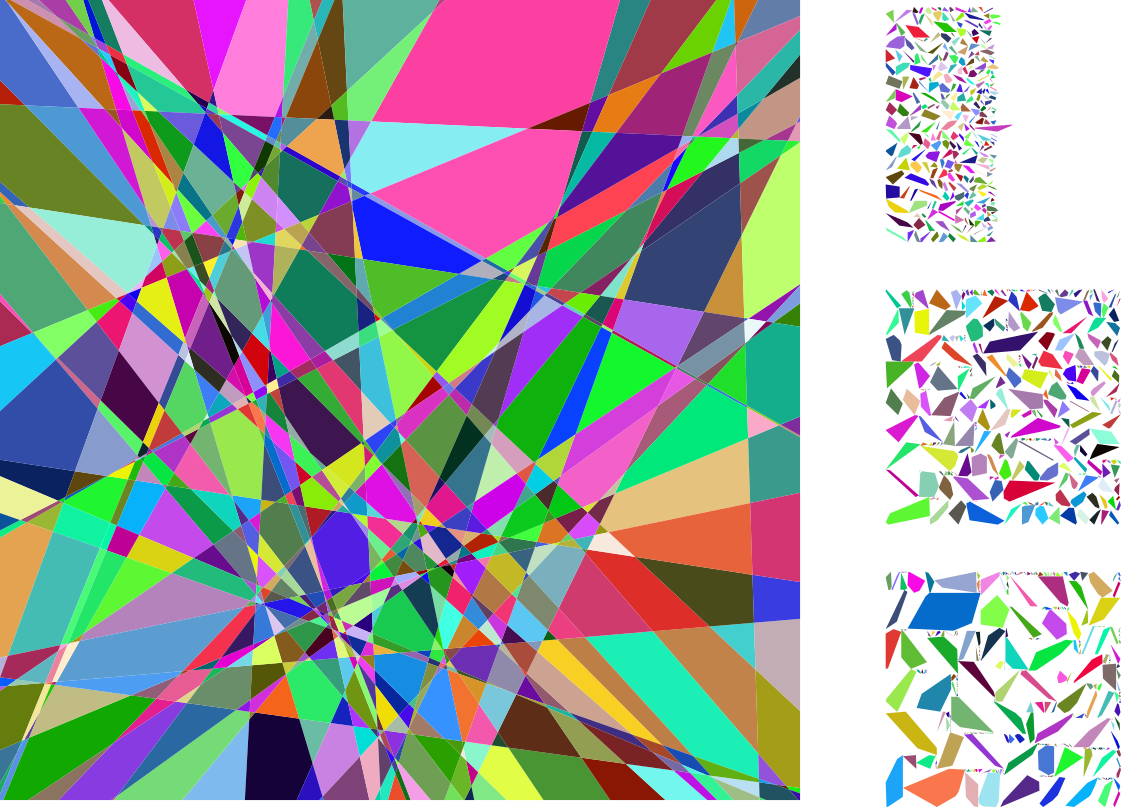
\includegraphics[scale=0.4]{img/scanLineTest}
\caption{Test du solveur "first-fit" ScanLineSolver}
\label{la banane}
\end{figure}



\newpage
\subsection{Outer}

La dernière étape de l'exécution a pour objectif d'écrire un fichier SVG contenant toutes les formes sélectionnées par l'utilisateur, après leur traitement par la classe \texttt{Solver}. Ceci est réalisé par la classe \texttt{Outer}, qui, à partir des formes précédemment déplacées par le \texttt{Solver} et de leurs identifiants récupérés par la classe \texttt{Parser}, va recopier les éléments associés à ces identifiants sur la sortie standard.\\

On parcourt donc l'arborescence du fichier SVG, en utilisant rapidXML, de manière à sélectionner les éléments en fonction de leur identifiant, pour ensuite ajouter (ou de modifier si le champ existe déjà) un champ contenant la matrice de transformation associée au déplacements effectués lors du packing.\\

Dans le cas d'une duplication (en bas de page), tous les éléments de l'arborescence parsés lors du parcours sont d'abord recopiés sans être modifiés, puis leur version modifiée est ajoutée si leur identifiant est reconnu comme élément à packer. On écrit ensuite sur la sortie standard le texte correspondant au fichier SVG ainsi généré, qui sera récupéré par le plugin ou par l'utilisateur pour être écrite dans un fichier.



\newpage
\section{Annexe}

\paragraph{Close Enough Script Language\\}

\setlength{\grammarparsep}{20pt plus 1pt minus 1pt} % increase separation between rules
\setlength{\grammarindent}{12em} % increase separation between LHS/RHS 
\begin{grammar}
<string> ::= [\verb|^|,()=]$^+$

<value> ::= int \alt double \alt <string>

<parameter> ::= <string> '=' <value>

<parameter\_list> ::= <parameter> \alt <parameter> ',' <parameter\_list> \alt $\epsilon$

<transformer> ::= "SimpleTransformer" \alt "HoleTransformer" \alt ...

<solver> ::= "LineSolver" \alt "MultilineSolver" \alt ...

<function> ::= <transformer> \alt <solver>

<instruction> ::= <function> '(' <parameter\_list> ')' ';'

<block> ::= <instruction> \alt "BEGIN" <instruction>$^+$ "END"

<big\_block> ::= <block> \alt "DO" int "TIMES" <block>

<program> = <big\_block>$^*$
\end{grammar}

\end{document}                                                                                                                                                                               





